%%%%%%%%%%%%%%%%%%%%%%%%%%%%%%%%%%%%%%%%%%%%%%%%%%%%%%%%%%%%%%%%%%%%%%%
%% Main Document
%%%%%%%%%%%%%%%%%%%%%%%%%%%%%%%%%%%%%%%%%%%%%%%%%%%%%%%%%%%%%%%%%%%%%%
\documentclass[a4paper,11pt]{report}

% General  instructions / Best Practice Rules:
% ------------------------------------
% * Only one sentence per line!
% * Use active voice whenever possible! ("we have investigated" instead of "it
%   was investigated")
% * Use past progressive instead of simple past! ("Banks et al. have shown"
%   instead of "Banks et al. showed")
% * Mark open points with \todo{ <Name of assigned person>: ... }
% * Only commit after checking that it compiles. 
% * Use \cref{<label>} only, no \ref !
% * For abbreviations, always use the Glossaries package and \gls{<abbrv>} or
%   \glspl{<abbrv>} ! --> ensures that every abbreviation is introduced correctly


%%%%%%%%%%%%%%%%%%%%%%%%%%%%%%%%%%%%%%%%%%%%%%%%%%%%%%%%%%%%%%%%%%%%%%%
%% EIT Package and Language Settings
%%%%%%%%%%%%%%%%%%%%%%%%%%%%%%%%%%%%%%%%%%%%%%%%%%%%%%%%%%%%%%%%%%%%%%

% document with serif font
% use [de] option for German documents
%\usepackage{style-eit-latex/EIT}
%\usepackage[de]{style-eit-latex/EIT}

% use [pt] option for PT Sans without serif
\usepackage[pt]{style-eit-latex/EIT}
%\usepackage[pt, de]{style-eit-latex/EIT}


%%%%%%%%%%%%%%%%%%%%%%%%%%%%%%%%%%%%%%%%%%%%%%%%%%%%%%%%%%%%%%%%%%%%%%%
%% Custom Packages
%%%%%%%%%%%%%%%%%%%%%%%%%%%%%%%%%%%%%%%%%%%%%%%%%%%%%%%%%%%%%%%%%%%%%%
% Load \includegraphics command for including pictures (pdf or png highly recommended)
\usepackage{graphicx}
\graphicspath{ {./graphics/} }
\usepackage{longtable}
% Typeset source/pseudo code
\usepackage{listings}
\usepackage[acronym,indexonlyfirst,nomain]{glossaries}
\usepackage{datatool}

\setacronymstyle{long-short}
\makenoidxglossaries
%%%

\renewcommand*{\acronymname}{List of Abbreviations}
\newacronym{aws}{AWS}{Amazon Web Services}
\newacronym{gcp}{GCP}{Google Cloud Platform}
\newacronym{ec2}{EC2}{Elastic Compute Cloud}
\newacronym{s3}{S3}{Simple Storage Service}
\newacronym{rds}{RDS}{Relational Database Service}
\newacronym{iam}{IAM}{Identity and Access Management}
\newacronym{it}{IT}{Information Technology}
\newacronym{iaas}{IaaS}{Infrastructure as a Service}
\newacronym{paas}{PaaS}{Platform as a Service}
\newacronym{saas}{SaaS}{Software as a Service}
\newacronym{cli}{CLI}{Command Line Interface}
\newacronym{scp}{SCP}{Service Control Policies}
\newacronym{ou}{OU}{Organizational Unit}
\newacronym{acl}{ACL}{Access Control Lists}
\newacronym{ad}{AD}{Active Directory}
\newacronym{vpc}{VPC}{Virtual Private Cloud}
\newacronym{ami}{AMI}{Amazon Machine Image}
\newacronym{csp}{CSP}{Cloud Service Providers}
\newacronym{cisa}{CISA}{Cybersecurity \& Infrastructure Security Agency}
\newacronym{owasp}{OWASP}{Open Web Application Security Project}
\newacronym{idc}{IDC}{International Data Corporation}
\newacronym{devops}{DevOps}{Development and Operations}
\newacronym{api}{API}{Application Programming Interface}
\newacronym{smb}{SMB}{Small-to-Medium-Sized Businesses}
\newacronym{hr}{HR}{Human Resources}
\newacronym{ci}{CI}{Continuous Integration}
\newacronym{cd}{CD}{Continuous Delivery}
\newacronym{hippa}{HIPPA}{Health Insurance Portability and Accountability Act}
\newacronym{gdpr}{GDPR}{General Data Protection Regulation}
\newacronym{cis}{CIS}{Center for Internet Security}
\newacronym{pci-dss}{PCI-DSS}{Payment Card Industry Data Security Standard}
\newacronym{pci-ssc}{PCI-SSC}{Payment Card Industry Security Standards Council}
\newacronym{ml}{ML}{Machine Learning}
\newacronym{ide}{IDE}{Integrated Development Environment}
\newacronym{ssrf}{SSRF}{Server Side Request Forgery}
\newacronym{ebs}{EBS}{Elastic Block Store}
\newacronym{mfa}{MFA}{Multi Factor Authentication}
\newacronym{imds}{IMDS}{Instance Metadata Service}



%%%%%%%%%%%%%%%%%%%%%%%%%%%%%%%%%%%%%%%%%%%%%%%%%%%%%%%%%%%%%%%%%%%%%%%
%% Hyphenation
%%%%%%%%%%%%%%%%%%%%%%%%%%%%%%%%%%%%%%%%%%%%%%%%%%%%%%%%%%%%%%%%%%%%%%

% correct bad hyphenation here
\hyphenation{net-works semi-conduc-tor quad-ra-ture mat-ches trans-form meth-od}


%%%%%%%%%%%%%%%%%%%%%%%%%%%%%%%%%%%%%%%%%%%%%%%%%%%%%%%%%%%%%%%%%%%%%%%
%% Document Configuration
%%%%%%%%%%%%%%%%%%%%%%%%%%%%%%%%%%%%%%%%%%%%%%%%%%%%%%%%%%%%%%%%%%%%%%
% import global settings file
\input{includes/settings}

% TODO: add own settings here


%%%%%%%%%%%%%%%%%%%%%%%%%%%%%%%%%%%%%%%%%%%%%%%%%%%%%%%%%%%%%%%%%%%%%%%
%% Title and Document Information
%%%%%%%%%%%%%%%%%%%%%%%%%%%%%%%%%%%%%%%%%%%%%%%%%%%%%%%%%%%%%%%%%%%%%%

\begin{document}
% Title, author and other information:
\title{Security Checks in AWS Security Framework}

\author{Vakul Sharma}

\maketitle

%%%%%%%%%%%%%%%%%%%%%%%%%%%%%%%%%%%%%%%%%%%%%%%%%%%%%%%%%%%%%%%%%%%%%%%
%% Body Text
%%%%%%%%%%%%%%%%%%%%%%%%%%%%%%%%%%%%%%%%%%%%%%%%%%%%%%%%%%%%%%%%%%%%%%

% INSERT YOUR CONTENT HERE:
\clearpage
\section*{Declaration}
\text
I hereby declare that the work presented in this thesis work is entirely written by myself and that I have not used any other references and sources other than the listed ones.
I have marked all indirect and direct statements as
quotations that are from other sources.\\

\raggedright{Kaiserslautern, October 18, 2022}\\

\hfill \break
\raggedright{Vakul Sharma}


\cleardoublepage

\section*{Abstract}
\text
Cloud computing has been a comprehensive technology for more
than two decades supporting
businesses of all sizes around the world.
A recent survey by International Data Group showed that 69\%
of businesses are using cloud technology already, and
18\% plan
to implement cloud-computing solutions.
The high volume of data generated by the organizations flows to the cloud.
This opens the door for accidental or malicious leaks of sensitive data.
Malicious actors such as attackers or hackers exploit vulnerabilities associated with cloud security to exfiltrate essential data and information for profit or other purposes from the organization’s network \cite{1}.

\hfill \break

Securing data is not just a process of protecting data
from unauthorized users, but it is an act of preventing
the data from destruction, modification, or
unauthorized access.
Cloud services provide numerous features that make accessibility of data a lot easier for the developers, but at the same time introduce many unauthorized access issues.
Due to these reasons, enterprises must think
about strengthening
their network security to avoid such unauthorized access that leads to service disruption and sometimes causes reputation damage \cite{1}.

\hfill \break
The main outcome of this thesis work is to highlight a
few security vulnerabilities in \gls{aws} namely
\gls{ec2}, \gls{iam},
\gls{s3}, \gls{rds}, and Lambda, and assess them using a
security assessment framework called Prowler.
Prowler is an open-source AWS CLI tool for auditing, security best practices assessment, forensics readiness, and hardening.
Security frameworks protect a user’s account against security vulnerabilities.
Prowler, a market-leading security tool performs the assessment of security vulnerabilities in AWS accounts.
It helps organizations to implement practices that ensure a secure and protected environment in place.
At the end of this thesis work, the efficiency of Prowler is evaluated and compared against other security tools.

\cleardoublepage


\section*{Zusammenfassung}
\text
Cloud Computing ist seit mehr als zwei Jahrzehnten eine revolutionäre Technologie, die Unternehmen aller Größen unterstützt.
Eine kürzlich von der International Data Group durchgeführte Umfrage ergab, dass 69 \% der Unternehmen bereits Cloud-Technologie verwenden und 18 \% planen, Cloud-Computing-Lösungen zu implementieren.
Die große Menge an Daten, die von den Organisationen generiert werden, fließen in die Cloud.
Dies öffnet die Tür für versehentliche oder böswillige Lecks sensibler Daten.
Böswillige Akteure wie Angreifer oder Hacker nutzen Schwachstellen im Zusammenhang mit der Cloud-Sicherheit aus, um wichtige Daten und Informationen für Profit- oder andere Zwecke aus dem Netzwerk der Organisation herauszuschleusen \cite{1}.


Das Sichern von Daten ist nicht nur ein Prozess zum Schutz von Daten vor unbefugten Benutzern, sondern auch ein Akt, um unbefugten Zugriff, Änderung oder Zerstörung von Daten zu verhindern.
Cloud-Dienste bieten zahlreiche Funktionen, die den Zugriff auf Daten für die Entwickler erheblich erleichtern, gleichzeitig aber viele Probleme mit unbefugtem Zugriff einführen.
Tatsächlich müssen Unternehmen die Stärkung ihrer Netzwerksicherheit überdenken, um solche unbefugten Zugriffe zu vermeiden, die zu Dienstunterbrechungen führen und manchmal Reputationsschäden verursachen \cite{1}.


Das Hauptergebnis dieser Diplomarbeit besteht darin, einige Sicherheitslücken in \gls{aws} nämlich
\gls{ec2}, \gls{iam},
\gls{s3}, \gls{rds}, und Lambda, hervorzuheben und sie mit einem Sicherheitsbewertungs-Framework namens Prowler zu bewerten.
Prowler ist ein Open-Source-AWS-CLI-Tool für Auditing, Best-Practice-Sicherheitsbewertung, Forensikbereitschaft und Härtung.
Sicherheitsframeworks schützen das Konto eines Benutzers vor Sicherheitslücken.
Prowler, ein marktführendes Sicherheitstool, führt die Bewertung von Sicherheitslücken in AWS-Konten durch.
Es hilft Organisationen, Praktiken zu implementieren, die eine sichere und geschützte Umgebung gewährleisten.
Am Ende dieser Diplomarbeit wird die Leistungsfähigkeit von Prowler bewertet und mit anderen Sicherheitstools verglichen.

\cleardoublepage

\section*{Acknowledgement}
\text I would like to thank my thesis supervisors, Jan Wennrich, and Mohammad Reza Gashtil, for their valuable assistance, useful critiques, time, and suggestions during the thesis.
His willingness to give me constructive advice has been very much appreciated.
\\
I’m also highly grateful to Prof.
Dr.-Ing Wolfgang Kunz for allowing me to do my thesis.
I would like to extend my thanks to my family members,
for their enthusiastic encouragement, and to all my
friends for their motivation.

\cleardoublepage

\tableofcontents

% Bei einem ungünstigen Seitenumbruch im Inhaltsverzeichnis, kann dieser mit
% \addtocontents{toc}{\protect\newpage}
% an der passenden Stelle im Fließtext erzwungen werden.



%! Author = vsharma
%! Date = 25.09.2022
% !TeX spellcheck = en_EN

\chapter{Introduction}

\par Cloud computing is in continual development to make different levels of on-demand services available to customers.
It helps companies reduce operating costs while increasing efficiency.
Organizations are continuously moving their technical assets to cloud, due to the continued proliferation of AWS. Despite several advantages offered by cloud computing, it also fosters security concerns that hamper the fast rate of adoption of cloud computing.
Enterprises should
be aware about the security challenges
faced
by
cloud computing before implementing to cloud
computing by expanding their
on-premises
infrastructure.
Even though cloud computing highly benefits people,
security has been the biggest challenge in cloud.
Comprehending the security threats and countermeasures will help organizations carry out the cost-benefit analysis and impulse the organizations to shift to the cloud.
To provide the cloud users better quality of service, security flaws must
be identified.
Many security vulnerabilities exist in cloud, and hackers
continue exploiting these security holes.
There is a glaring need for a tool that provides a comprehensive and structured approach to pen-testing AWS vulnerabilities by the offensive security community \cite{2}.

\section{Motivation}
\par Cloud computing has become a
popular subject in computer science and software
engineering in recent years.
With low maintenance costs, flexibility, ease of
deployment, cost-effective scalability, and overall aid in efficiency, businesses, and IT leaders all over the world are replacing legacy, classic on-premises data center technology with cloud-based solutions.
As cloud computing offers beneficial characteristics like
on-demand provisioning and billing against the actual
consumption of computing resources, enterprises leverage
these advantages by migrating their costly and legacy
infrastructures such as servers, firewall appliances,
databases, or their software and hardware solutions that
are not operating at the optimum capability to the cloud
such as Microsoft Azure, IBM Cloud, Amazon Web Services
(AWS), Alibaba Cloud, Google
Cloud Platform (GCP), or other third-party cloud vendors.
Cloud migration promises cost benefits and agility and it opens the way for the future.
The pandemic fast-tracked the shift to cloud technology by upending how organizations worked and operated.
The lockdown compelled people to work from their homes using conferencing and collaboration services \cite{2}.


\par Cloud computing provides 3 as-a-service offerings
namely PaaS abbreviated as Platform as a Service,
SaaS abbreviated as Software
as a Service
(SaaS), and IaaS abbreviated as Infrastructure
as a
Service
(IaaS).
These cloud
services help enterprises to scale and adopt powerful cloud offerings such as computing and storage capabilities.
The enterprise doesn't need to bear the cost and overhead
of purchasing and maintaining the IT infrastructure in its
data center and can access and scale its IT capabilities at
an anticipated cost.
The term \textit{as a service} refers to the way the IT assets are consumed and shows the major difference between traditional IT and cloud computing.
In traditional IT, a company consumes IT assets such as system software, hardware, applications, and tools.
The company purchases these IT assets and maintains them within the company’s on-premises data center.
In cloud computing, these IT assets are owned, managed,
and maintained by the cloud service providers, the enterprise can use only the infrastructure needed to create the development environment, scale the environment up or down as long as they need, and then stop when finished, paying only for the resources used. This helps enterprises to match the current world demand and reduces expenses \cite{3}.

\par Though cloud migration may seem intimidating at
first, if the preparation is done correctly, it will lead to a smooth migration.
While cloud migration brings greater opportunities, it introduces its own challenges.
These challenges are associated with security controls
that the enterprise built for its on-premises environment.
Security control needs to rebuild, making use of the cloud services to replace traditional on-premises security measures.
When migrating to the cloud for the first time, the required expertise might not be available within the organization.
Another biggest challenge of migrating the application to the cloud is to protect sensitive business data against attacks.
The application migration is oriented mainly toward moving the application into the cloud.
However, legacy applications need a more sophisticated migration mechanism to find out the most suitable cloud environment and fully leverage the benefits of cloud computing \cite{4}.

\par Compliance and security are shared responsibilities between AWS and the customer.
The shared security responsibility model distributes these
responsibilities between the customer and the cloud
service providers.
The security team of the customer maintains the
responsibilities for security as they move applications,
containers, data, and workloads to the cloud, while the
cloud service provider takes some responsibility, but not
all, thus reducing the workload for the customer.
However, this notion of shared responsibility can be misunderstood and can result in the assumption of the cloud
workloads, as well as any data, applications, or activity associated with them are fully protected by the cloud provider \cite{5}.



\par FlexBooker, an online booking software was hacked on
December 23, 2021, \cite{6}\cite{7}.
This hacking resulted in the looting of approximately 3
million
users personal information such
as driver's license data, etc.
FlexBooker hosted its application and services in the AWS cloud, using computing and storage instances.
The data was exposed due to an improperly configured S3 bucket \cite{8}.
Amazon S3 is a storage service that AWS offers, and it
stores objects within buckets.
These objects represent a file and its descriptive metadata \cite{9}.




\par  To protect users from such security attacks, several security frameworks exist that aims to strengthen the
security of users account.
These frameworks provide a list of controls and are recommended with different cloud services and
configurations.
But such frameworks do not always provide in-depth security controls for the services.
Cloud
environments assessed through such frameworks might still have gaps and are vulnerable to attacks.
The reason is simple, these frameworks are not
derived from vulnerability data or actual exploits \cite{10}.

\par This research work aims at identifying the competency of a security framework named \textit{Prowler}.
It runs security checks and performs assessments of different security vulnerabilities such as misconfiguration,
server-side request forgery, etc.
This thesis focuses on different AWS services such as
\gls{ec2}, \gls{rds},
\gls{iam}, Lambda, and \gls{s3}.
The
framework assesses different vulnerabilities that occur on the mentioned AWS services.



\section{Goals}
\par In this regard, the goal of this thesis is to acquaint users with different security vulnerabilities in AWS
services.
These security vulnerabilities are assessed using an assessment tool called \textit{Prowler}. The
efficiency of assessment done using Prowler is determined using 2 approaches. In the first approach, test scenarios
are developed to verify the assessment results for each check in Prowler. For the second approach, an open-source
application is used and an assessment of the security vulnerabilities within the AWS account is done.

\par In the end, the assessment of security vulnerabilities performed using Prowler is compared to the assessment performed by other security assessment tools \textit{ScoutSuite}.

\par For example, if we have an AWS account with a public S3 bucket, it is a security vulnerability and can lead to a data breach.
By using Prowler, it is possible to identify such security vulnerabilities and thus limit the risk of security attacks.

\section{Contribution and Thesis Outline}
\par The thesis contributions are:
\begin{itemize}
    \item Identify the security vulnerabilities in AWS services.
\end{itemize}
\begin{itemize}
    \item Perform the security vulnerability assessment using Prowler.
\end{itemize}
\begin{itemize}
    \item Compare the result of the assessment done using Prowler against ScoutSuite.
\end{itemize}
\begin{itemize}
    \item Determine the efficiency of Prowler against the identified security vulnerabilities.
\end{itemize}

\par This thesis is organized as follows:
\par \textbf{Chapter 2 (Related Work)}: This chapter briefs about:
\begin{itemize}
    \item Cloud computing: The basics of cloud computing,
    its types, and the different types of cloud services
    namely IaaS, PaaS, and SaaS.
\end{itemize}
\begin{itemize}
    \item Amazon Web Services (AWS): A detailed
    background about Amazon Web Services (AWS) and AWS
    services such as RDS, Lambda, S3, etc.
\end{itemize}
\begin{itemize}
    \item Security framework: Information about security
    framework basics and an open-source security assessment tool, Prowler is described.
\end{itemize}

\par \textbf{Chapter 3 (Problem Statement)}: In this chapter, different security vulnerabilities identified in five
AWS services are highlighted.
A piece of detailed information about each of the identified security vulnerabilities is also provided in this chapter.
\par \textbf{Chapter 4 (Methodology)}: This chapter describes the approaches to determine the efficiency of prowler.
\begin{itemize}
    \item Using Test Driven Approach: The manual approach of developing test cases to determine the efficiency of Prowler.
\end{itemize}
\begin{itemize}
    \item Using Open-Source Application: Evaluate the efficiency of Prowler by deploying an open-source
    application on AWS.
\end{itemize}
\par In the end, another open-source tool ScoutSuite is
described, and an AWS account is assessed using ScoutSuite.

\par \textbf{Chapter 5 (Evaluation)}: This chapter provides
\begin{itemize}
    \item The result of the assessment performed using the two approaches mentioned in chapter 4.
\end{itemize}
\begin{itemize}
    \item Comparison between the assessment of the open-source application using Prowler and ScoutSuite.
\end{itemize}
\par \textbf{Chapter 6 (Conclusion and Future Work)} concludes this thesis by summarizing the work done, results obtained, open topics, and future work.


%! Author = vsharma
%! Date = 25.09.2022
% !TeX spellcheck = en_EN

\chapter{Related Work}

\section{Cloud Background}

\subsection{Cloud Computing}
Cloud computing in simple terms is defined as the delivery of computing services and resources.
These include
storage, databases, servers, software, and networking over the internet.
Cloud computing is a combination of two
words “cloud” which means “internet” and computing involves the systems and infrastructures that enable a computer to run and build, deploy, or interact with information.
Cloud computing is a very common phrase that people hear nowadays but might not actually understand.
It is because cloud computing encompasses several different services and systems thus making it ambiguous or confusing. In simple words, cloud computing can be defined as the delivery of computing services, these include databases, storage, servers, etc. over the internet \cite{11}.

Cloud computing enables the use of off-site systems which helps the computers to store, manage, process, and
communicate information.
These services are not posted on-premises by the
organization rather they are accessible over the internet.
These systems can store anything from software programs to email servers, data storage, etc \cite{11}
\cite{12}.

\subsection{Types of cloud computing:}

\par There are different cloud providers that offer cloud services namely Amazon Web Services (AWS), the cloud computing service of Amazon.com, Microsoft Corporation’s cloud segment contains Azure, Google Cloud Platform (GCP), part of Alphabet Inc, etc.
Each of the cloud platforms is unique in its own way and offers a plethora of options for organizations to select from based on their specific requirements.
When considering the services offered by these clouds,
Google Cloud offers up to 60+ services, whereas Azure
offers around 100+ services.
AWS, on the other hand, offers around 200+ services.
In terms of the availability zones, AWS has 66
availability zones, Azure has 54 regions worldwide and is
available in 140 countries all around the world, and
\gls{gcp} has been made available in
20 regions around the world \cite{13}.
While deciding on a cloud service provider there are
several factors that needs to be considered.
In order to determine the most suitable type of cloud computing on which the cloud services can be implemented, it is better to first identify the type of cloud computing architecture or cloud deployment.
There are three different cloud offerings to deploy cloud services: a private cloud, a public cloud, or a hybrid cloud \cite{14}.
\hfill \break
\textbf{Private cloud:}
Private cloud refers to computing resources that are used by a particular organization or a single business.
In this,
the computing resources are owned, operated, and governed by the same organization.
The cloud
computing resources are physically located at the
organization’s on-site datacenter in the private cloud, the
services
and
the
infrastructure are maintained by a private network \cite{14}.
\hfill \break
\textbf{Public cloud:}
This type of cloud usually offers B2C (Business to Consumer) type of interactions. Public clouds are operated and
owned by a third-party cloud service provider which delivers these resources over the internet. AWS is an example of
a public cloud where the cloud service provider owns and manages all the software, hardware, and other supporting
services \cite{14}.
\hfill \break
\textbf{Hybrid cloud:}
A hybrid cloud refers to the mixed storage, services, and computing environment comprises of a public cloud such as
AWS and an on-premises infrastructure, a private cloud. The hybrid cloud approach is the most widely used infrastructure configuration these days as it enables the organization
to continue using their on-premises servers while taking the advantage of available public cloud options like AWS,
and Azure. This enables the organization to comply with the data residency policies while leveraging the benefits and
security of the public cloud \cite{14}.


\subsection{Types of cloud services:}
\textbf{Infrastructure as a service (IaaS)}
\par This type of cloud computing service offers
essential storage, memory, compute, and related networking, such as
operating systems and databases, as a cloud service to replace the on-premises infrastructure.
In a typical IaaS
architecture, the most essential components are hosted by the cloud providers such as Networking hardware, Servers, Storage, Physical hardware, etc. This feature enables IaaS to provide the same capabilities and technologies as offered by the traditional on-premises data centers \cite{9}. The customer needs to only perform a few steps:
\begin{itemize}
    \item Customers can access the services over the internet by logging in to the IaaS platform created by the cloud
    service provider \cite{15}.
\end{itemize}
\begin{itemize}
    \item The customer is then required to create a Virtual
    Machine (VMs) on the cloud platform according to their
    requirements and then install the operating system
    (OS) on the VMs. Once the OS is deployed on the VM,
    the customer must deploy middleware, create
    storage buckets to hold the workloads and backups, and
    install the enterprise workload into that VM \cite{15}.
\end{itemize}
\begin{itemize}
    \item Finally, these VMs can be deployed along with databases, apps, desired tools, and the company’s workload \cite{15}.
\end{itemize}
IaaS benefits businesses by reducing operating costs, and by spending less on software upgrades and maintenance
\cite{15}.

\begin{figure}
    \centering
    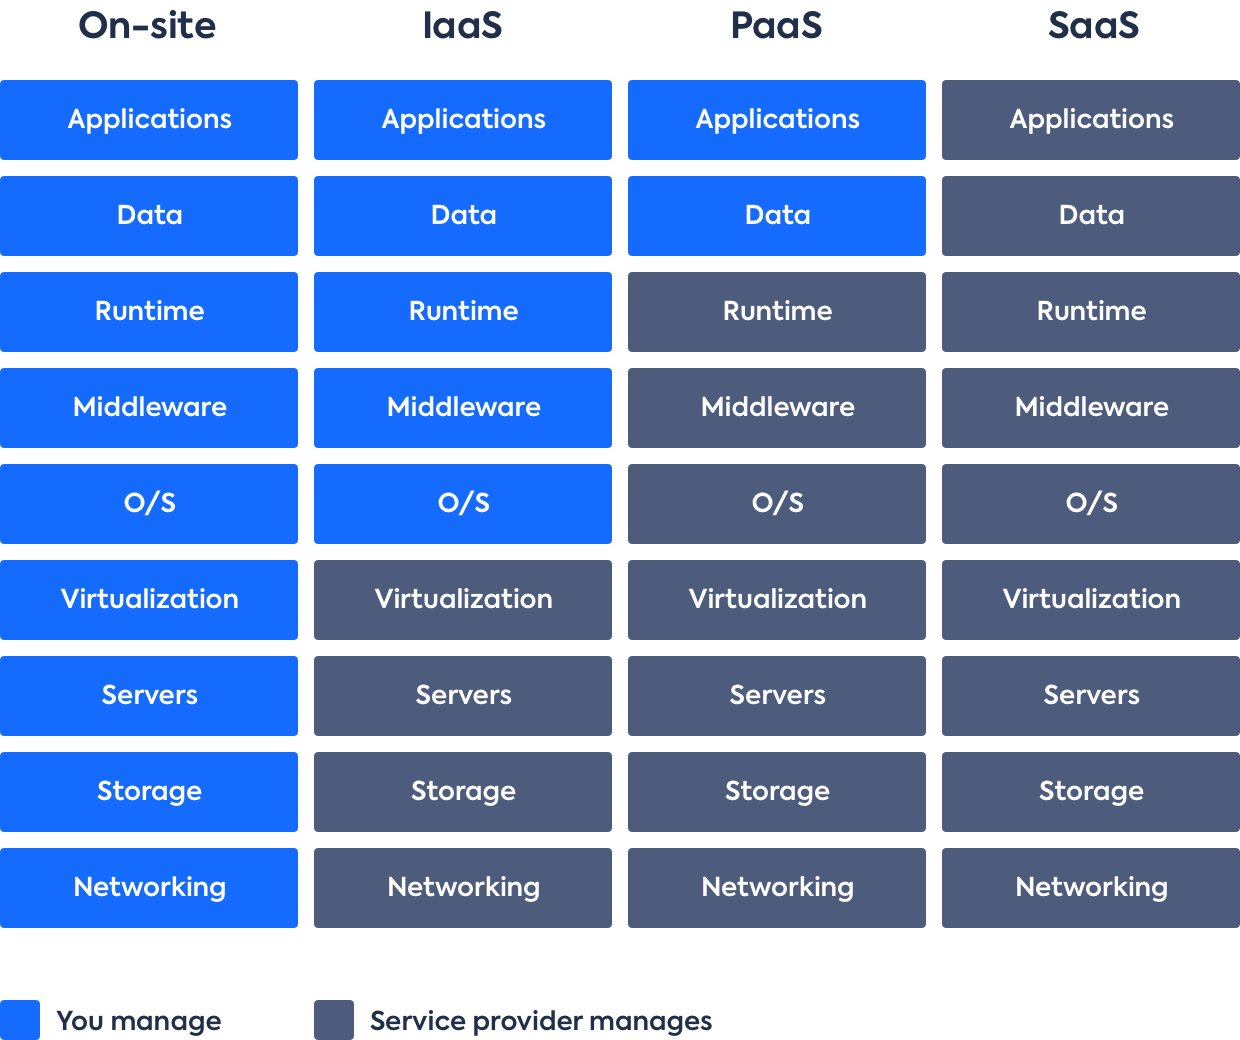
\includegraphics[width=\textwidth]{iaaspaassaas.jpg}
    \caption{Cloud computing models}{\cite{16}}
    \label{fig:iaaspaassaas}
\end{figure}

\clearpage
\textbf{Platform as a service (PaaS)}
\par \gls{paas} is a model that provides cloud-based
services
enabling the developers and businesses to build software
and applications at a faster speed that could not be
achieved in on-premises solutions.
It is an on-demand service providing companies with a
complete set of software, hardware, and infrastructure for
developing, running, testing, and managing software
applications and eliminates the complexity and expense of
buying, evaluating, configuring, and managing all the
required software and hardware needed for applications.
It provides the organization with a cost-effective,
complete, and flexible platform.
It allows programmers to develop web and mobile
applications without worrying about managing or setting up the underlying infrastructure for storage, servers, databases, and networks that are needed for deployment \cite{15}.


\par With PaaS, the organization avoids the complexity and expense of buying the software licenses, the underlying infrastructure, container orchestrators, development tools, and middleware or other resources.
The organization only manages the application developed
by them and cloud service providers such as Amazon AWS
manage everything else \cite{15}.\\

\hfill \break

\textbf{Software as a service (SaaS)}
\par \gls{saas} is a method of delivering software and
application
to the end user over the internet.
These applications can be accessed via the
mobile application, internet browser, or desktop app.
Common examples of SaaS are calendaring, email, and office tools (such as Microsoft Office 365).
It is a distribution model in which the applications are hosted by cloud service providers or vendors to users across the globe.
The another name given to these applications are
on-demand
software, Web-based software, or hosted software and run
on the provider's servers.
The provider takes all the responsibilities of managing the application that includes performance, availability and security.
SaaS offers a subscription-based model
which
means users pay recurring monthly or annual fees for
using the product, the user don’t need to worry
about the huge
upfront cost.
In SaaS, all the
application software, middleware, application data, and infrastructure are in the cloud service provider’s data center.
The software and hardware are managed by the cloud
service provider.
The cloud service provider also ensures the security and availability of applications and data.
It enables bringing up the organization’s application and
running quickly and at a minimal upfront cost \cite{15}.

\par Figure \ref{fig:iaaspaassaas} describes the responsibilities of each deployment model compared to the on-premises setup.

\section{Amazon Web Services}
\par This section introduces the relevant AWS services and associated terminology used in this thesis. It is written to provide the reader with ample background knowledge required to understand this research work. It therefore by no means introduces the entire AWS platform.

\subsection{General AWS background}

\par Amazon web services is an evolving cloud computing subsidiary of Amazon.
Amazon Web
Services portfolio comprises more than 200+ services including database, compute, application
development, security, infrastructure management, analytics, migration, etc.
that help the
organization to scale and grow.
For example, AWS provides a wide range of databases that are
designed specifically for specific applications.
AWS combines the offerings of the three cloud services 
namely PaaS, IaaS, and SaaS \cite{17}.

\par AWS was launched in 2006 and was one of the first
cloud service providers to introduce a pay-as-you-go cloud computing model. It offers various tools and solutions for developers \cite{18}.

\par AWS cloud infrastructure is a highly secure,
reliable, and extensive cloud platform \cite{19}. Whether
it is required to deploy the application workloads
globally with just one click, or to develop and deploy specific applications closer to the end user with latency in the single-digit millisecond range, AWS offers the right cloud infrastructure anywhere, anytime \cite{20}.

\begin{itemize}
    \item AWS Regions
    \item Availability zones
    \item Edge locations
\end{itemize}

\begin{figure}
    \centering
    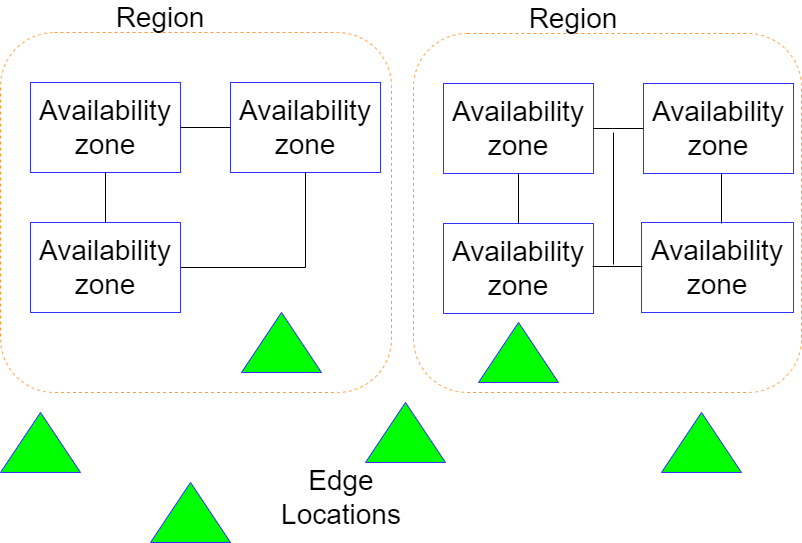
\includegraphics[width=\textwidth]{geographicalcomponents.png}
    \caption{AWS Geographical Components}{\cite{16}}
    \label{fig:identities}
\end{figure}

\par When designing and architecting the cloud infrastructure it is very important to know where the instances, services are data are located.
This is a fundamental criterion to implement a highly
available and scalable network that offers low latency
\cite{20}.


\textbf{Region}
\par Regions are geographical locations to operate and run cloud services.
These regions are spread globally and reduce the latency incurred by the customer when accessing the resource.
Each AWS region contains availability zones.
For each AWS region, there are a minimum of 2 Availability
Zones and a
maximum of 6 Availability Zones, however typically 3 or more are usually found.
The regions are connected to one another via a high-speed
fiber network and are isolated from each other \cite{21}


\textbf{Availability zones}
\par Each region is made of a logical building block known as \textit{AWS Availability Zone (AZ)} and is isolated from the failures of other availability zones.
The AWS regions operate independently and are isolated from other regions, but the availability zone within a region provides low-latency network connectivity to other Availability Zones within the same AWS Region.
There is no explicit cost incurred for the network connectivity between two Availability Zones within the same AWS Region.
Depending on the service used, in case of a failure, if an Availability Zone goes down, it is possible to ensure high availability by shifting the workload to another Availability Zone within the same region, this capability is known as \textit{Multi-AZ} redundancy.
The figure \ref{fig:identities} shows 2 different AWS
regions which are isolated from each other and each region consists of AWS Availability Zones \cite{22}.

\textbf{Edge Location}
\par In order to reduce the latency for the traffic, edge locations are deployed at multiple locations across the
world. Edge locations limit to building a new data center
if the customers are in different cities, a different
state, a different
country or a different
part of the world. Edge locations can be understood as servers that are placed geographically close to the clients.
If we consider an example, an organization has many clients in Tokyo accessing the information which is deployed in a
region in Mumbai. In such cases, instead of clients sending requests constantly to Mumbai region for accessing the
information, we can cache a copy of the relevant information in Tokyo. Amazon CloudFront allows delivering video,
information, APIs to clients, or applications across the world. AWS CloudFront uses edge locations for accelerating
communication with customers \cite{23}.

\subsection{Services}

\textbf{AWS Identity and Access Management (IAM)}

\par Amazon \gls{iam} is a web service that helps to
securely
control access for the users to Amazon Web Services resources and services.
Using IAM enables creating and managing Amazon Web Services groups and users and uses permissions to allow and deny their permissions to AWS resources.
IAM enables organizations to create and control services
for user authentication or limit access to a certain set of people who use their AWS resources \cite{24}.


\par When an AWS account is created, it begins with one
sign-in identity.
This identity has
complete access to all AWS resources and services in the account and is called the \textit{root user}.
The AWS account root
user is accessed by signing in with the email address and password that you used to create the account.
As
recommended, the usage of root users must be avoided for
everyday tasks \cite{25}.


\begin{figure}
    \centering
    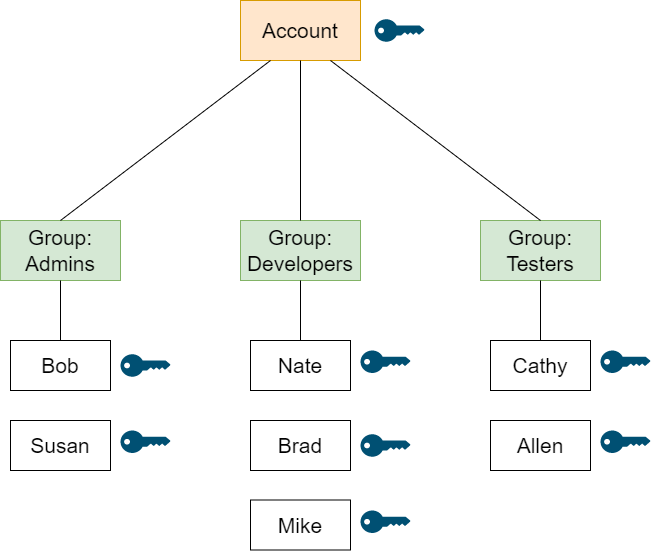
\includegraphics[width=\textwidth]{groupusers.png}
    \caption{IAM users and groups}{\cite{26}}
    \label{fig:groupusers}
\end{figure}

\textbf{IAM Users}

\par An IAM user represents an entity within the AWS account.
This entity corresponds to an application or a person and has specific permissions.
Users have their own set of authentication parameters such as access key, secret key, or password that is required to access the AWS account through CLI or AWS console.
An IAM user does not always represent an actual individual.
Each IAM user is associated with only one AWS account
\cite{27}.
\hfill \break

\textbf{IAM Group}
\par An IAM group is an identity that specifies a 
collection of IAM users as shown in figure \ref{fig:groupusers}.
The user
groups help in specifying the permissions for multiple users, thus making it easier to manage the permissions for the users.
For example, there could be a user group in an organization called Admins that provides all users administrator permissions who belong to that user group.
A user belonging to a user group gets assigned all the permissions that are assigned to the user group automatically.
If a new user joins the organization and should have administrator privileges, just by adding the new user to the admin user group, the user can be assigned the required permissions.
Similarly, if a user changes a job role within the organization, instead of editing that user’s permissions, it is possible to simply remove them from the old user groups and add them to the new user groups \cite{27}.
\hfill \break


\textbf{Roles}
\par An IAM role is not associated with a specific person,
but it is similar to an IAM user.
A role can be assumed
temporarily by switching the roles in the management
console of AWS. It is also possible to assume a role
through the AWS API operation or by calling the AWS
\gls{cli}
or by using a custom URL. However, a role is intended to be assumable by anyone who needs it instead of being uniquely associated with one person.
There are no standard long-term credentials such as passwords or access keys associated with a role. Instead, when a role is assumed, it provides temporary security credentials for the role session. It is possible to use roles to delegate access to users, services, or applications that don't have access to your AWS resources. For example, it is required to grant users within an AWS account access to resources the users usually don’t have or grant users in one AWS account access to resources in another account \cite{27}.

\hfill \break
\textbf{Policy}

\par An IAM policy is an IAM entity that sets permission and controls access to AWS resources.
The IAM policies are attached to AWS resources or IAM identities (users, groups, or roles) and define their permission.
These policies are evaluated when a principal such as a role or a user makes a request. Most policies in AWS are stored as JSON documents. IAM policies define permissions which specify who has access to the resources and what operation they can perform. For example, if there exists a policy that allows the GetUser action, then if this policy is assigned to the user, the user would be able to fetch the information either by using the AWS API or the AWS CLI or the AWS Management Console \cite{14}.

\par AWS provides six types of policies:

\begin{itemize}
    \item \textbf{Identity-based policies:} Identity-based policies are JSON documents that control what actions an
    identity
    (users, groups, and roles) can perform, under what conditions, and on which resources \cite{27}. The Identity-based policies can be further categorized as:
    \begin{itemize}
        \item Managed policies: Standalone identity-based policies that are attached to multiple users, groups, and
        roles in an AWS account \cite{27}.
    \end{itemize}
    \begin{itemize}
        \item Inline policies:  Policies that are added directly to a single identity such as user, group, or role.
        Inline policies maintain a strict one-to-one relationship between an identity and a policy and are deleted when the identity is deleted \cite{27}.
    \end{itemize}
\end{itemize}

\begin{itemize}
    \item \textbf{Resource-based policies:} Policy document attached to a resource such as an Amazon S3 bucket is known as Resource-based policies.
    These are inline policies and grant the specified permission to perform specific actions on a resource \cite{27}.
\end{itemize}
\begin{itemize}
    \item \textbf{IAM permissions boundaries:} A permissions' boundary sets the maximum permissions that can be granted to an IAM entity by an identity-based policy.
     When the permissions boundary for an entity is set, the entity can perform only the actions that are allowed by both its permissions boundaries and its identity-based policies.
     Permissions boundary does not limit the
    resource-based policies that specify the user or role as the principal \cite{27}.
\end{itemize}
\begin{itemize}
    \item \textbf{Organizations \gls{scp}:} Amazon
    Organizations
    is a service for grouping and centrally managing the Amazon accounts that the business owns.
    It helps to centrally manage and govern the environment as the organization grows and scales its AWS resources.
    The maximun permission for account members of an
    \gls{ou} is defined using
    Amazon
    Organizations.
    AWS OSCP limits the permissions granted to entities i
    .e. users or roles within the account by the
    identity-based policies or resource-based policies,
    but it does not grant permissions \cite{27}.

\end{itemize}
\begin{itemize}
    \item \textbf{Access control lists (ACLs):} ACL is a service policy that allows to control the access to a resource by the principals in another account.
    ACLs are the only policy types that does not uses the JSON policy structure and are similar to resource-based policies.
    ACLs are used to grant permissions to the specified principal since they are cross-account permissions policies.
    Using ACL it is not possible to control the access within the same account \cite{27}.
\end{itemize}
\begin{itemize}
    \item \textbf{Session policies:} Session policies are
    policies used for programmatically creating a temporary session for a federated user or role by passing them as parameters.The intersection of session policies and identity-based policies for the IAM user or role represents the permissions for a session \cite{27}.
\end{itemize}

Figure \ref{fig:iamidentities} shows the overview of AWS IAM concepts in AWS infrastructure.


\begin{figure}
    \centering
    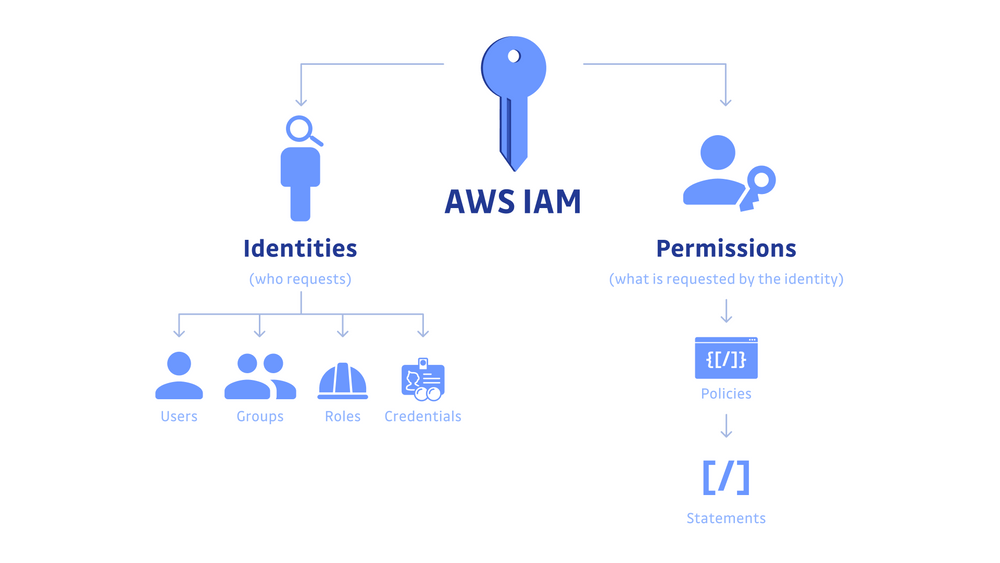
\includegraphics[width=\textwidth]{iaminfrastructure.png}
    \caption{Overview of AWS IAM concepts}{\cite{28}}
    \label{fig:iamidentities}
\end{figure}


\hfill \break

\textbf{Features of IAM}

\begin{itemize}
    \item \textbf{Granular permissions:} Based on the usage, permissions can be granted to different people to access
    different resources. For example, some users are granted complete access to Amazon DynamoDB ,Amazon S3, Amazon EC2, and other AWS services while other users are only
    provide permissions to administer some EC2 instances, read-only access to some S3 buckets but no other services \cite{27}.
\end{itemize}
\begin{itemize}
    \item \textbf{Multi-factor authentication (MFA):} To enable enhanced security of the AWS account, it is possible
    to enable
    two-factor authentication to the root account as well as to the individual users’ account. This ensures the AWS user along with providing the username and password for the account also provides a code from a configured device \cite{27}.
\end{itemize}
\begin{itemize}
    \item \textbf{Identity federation:} Identity federation is a system of trust between two parties used for the purpose of authenticating the users and sharing the information that is required for granting access to the resources.
    Users who have their password in the organization's
    corporate network or elsewhere such as in the
    internet identity provider are allowed to log in to the AWS console by the identity federation.
    For example, if there is a user who has logged into his
    google account and would like to use the AWS account,
    then identity federation helps AWS IAM to trust the authentication method.
    This authentication enables temporary access to the user’s AWS account \cite{27}.
\end{itemize}
\begin{itemize}
    \item \textbf{Password policy:} Password is used to authenticate a user’s account and a strict password policy
    can make it
    even more secure. IAM password policy allows for password rotation and resetting the password remotely. It is
    possible to set rules such as a password must contain a number, special characters, or special symbols \cite{27}.
\end{itemize}


\textbf{Amazon Elastic Compute Cloud (EC2)}

\par Amazon \gls{ec2} is one of the core services offered by
AWS
which
allows to rent virtual machine to run computer
applications. Amazon EC2 avoids upfront hardware setup investment, enabling faster development and deployment of applications. Amazon EC2 enables launching as few or as many virtual servers as needed, managing storage, and configuring security and networking. Amazon EC2 enables scaling uo or down based on the changes in the requirements or reduction in the need to forecast traffic, and spikes in popularity \cite{29}.

\par Amazon EC2 provides virtual server that are used for
running applications on the AWS infrastructure. This
virtual server is called an EC2 instance and they come in different configurations of storage, memory, CPU, and networking resources to suit user needs. EC2 instances can be used for any computing task, for example as a web server. An AWS user can create, launch, and terminate an instance based on the need, paying by the second for active servers and hence the term elastic. In order to provide high level of redundancy and optimize latency, Amazon EC2 provides users with control over the geographical location of instances. Placing all of the instances into the same AZ will likely give us the best latency between them. When an EC2 instance is provisioned, by default each instance is assigned automatically a DNS name and a public and private IPV4 address \cite{30}.


\textbf{Features of EC2}
\begin{itemize}
    \item \textbf{Elastic Web-Scale Computing:} Amazon EC2 enables users to expand the capacity as per their needs within minutes, not hours or days.
    Users can simultaneously commission one, hundreds, or even thousands of server instances.
    It is possible to run many servers in
    parallel
    with these instances.
    Amazon EC2, user can decrease or increase the
    automation as per their needs \cite{31}.
\end{itemize}

\begin{itemize}
    \item \textbf{Versatile cloud hosting services:} Amazon EC2 gives users the choice to select from a variety of instance types, operating systems, and software packages.
    Amazon EC2 allows selecting a configuration of memory, instance storage, CPU, and boot partition size that is optimal for your choice of operating system and application. For example, the operating system options include a variety of Linux variants as well as Microsoft Windows Server \cite{29}.
\end{itemize}

\begin{itemize}
    \item \textbf{Security:} Cloud security is the highest priority at AWS. Amazon works with the Amazon VPC to provide additional security, isolating resources, and robust networking for the compute resources.
    The compute instances in AWS are located in the VPC in the specific IP range.
    Further, the user decides which instances are exposed
    to the internet and which remain private \cite{31}.
\end{itemize}

\begin{itemize}
    \item \textbf{Conjunction with other Amazon web
    services:} Amazon EC2 collaborates with most AWS
    services such as Amazon RDS, Amazon VPC, Amazon SQS, and Amazon S3 to provide a complete, secure, comprehensive solution for
    computation, query processing, and cloud storage
    across a wide range of applications \cite{31}.
\end{itemize}

\begin{itemize}
    \item \textbf{Completely controlled:} Users have
    complete control over the instances including root
    access and the ability to interact with instances just like any other system. Users can stop the instance while keeping the data on the boot partition, and then restart it using web service APIs. Using web service APIs makes it possible to reboot the instances remotely \cite{31}.
\end{itemize}

\textbf{Amazon Machine Image (AMI)}

\par An Amazon Machine Image (AMI) is a maintained and
supported image provided by AWS. An AMI provides the necessary information required for launching an instance. An AMI must be specified while launching an instance. It is possible to launch multiple instances of the same configuration from a single AMI. When instances of different configurations need to be launched, different AMI must be used \cite{32}.

\begin{figure}
    \centering
    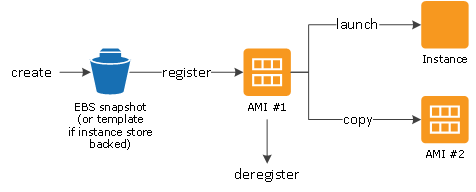
\includegraphics[width=\textwidth]{ami.png}
    \caption{Amazon Machine Image}{\cite{32}}
    \label{fig:ami}
\end{figure}

\par An AMI includes \cite{32}:
\begin{itemize}
    \item One or multiple Amazon \gls{ebs} snapshots or a
    template for the root volume of the instance, for instance-store-backed AMIs (for example, an application server, an operating system, and applications).
\end{itemize}
\begin{itemize}
    \item Launch permission in order to control which AWS accounts can use the AMI to launch instances.
\end{itemize}
\begin{itemize}
    \item A block device mapping that specifies to which instance the volumes must be attached when it’s launched.
\end{itemize}



\par Figure \ref{fig:ami} shows the lifecycle of AMI. The
Amazon Machine Image (AMI) is stored in an Amazon S3
bucket after it is created. This image is then registered and can then be used to launch a new instance. An AMI can be
copied to the same as well as to different AWS regions.
The AMI can be deregistered, if it is no longer required.
Upon deregistration a new instances cannot be launched
using the AMI, but the existing instances using AMI will
not be affected \cite{32}.

\par It is possible to launch an instance using an existing AMI. If the instance is customized, for example, the
software is installed on the image, this customized AMI can be saved with the updated configuration. Launching an
instance from this customized image contains customizations that were made earlier. To restrict the availability of
an AMI it can be made private, alternatively, the AMI is
made public when the access doesn’t need to be restricted \cite{33}.


\hfill \break

\textbf{Instance metadata and user data}
\par Instance metadata is the data associated with your EC2 instance that can be used to manage or configure the
running instance using the Instance metadata service (IMDS). Each EC2 instance has access to the Instance metadata
service (IMDS). The instance metadata is divided into different categories such as events, hostnames, and security
groups. Instance metadata service contains information
about the running EC2 instance and can be used to capture the temporary API credentials for accessing the AWS APIs \cite{34}.

\par Instance metadata can be used to access user data that is specified when launching the instance. For example, it
is possible to specify parameters for configuring the instance or include a simple script. It is also possible to
build generic AMIs and use user data to modify the configuration files supplied at launch time.
When more than one instance is launched at the same time,
the user data is available to all instances.
Each instance has a unique number called the ami-launch-index number.
This number allows for writing code that controls what to
do.
For example, the first host might elect itself as the original node in a cluster \cite{34}.


\hfill \break

\textbf{Amazon Relational Database Service (RDS)}

\par Amazon \gls{rds} is a set of managed services that
make it
easy
to
set up, operate, and scale databases in the Amazon Web Services Cloud.
Amazon RDS supports an array of database engines to organize and store data.
It also helps with relational database management tasks,
such as data backup, patching, recovery, and migration.
Amazon RDS provides its users access to the functionality of a familiar MariaDB, MySQL, SQL Server, Oracle, or PostgreSQL database.
It facilitates the deployment and maintenance of relational databases in the cloud.
Figure \ref{fig:rds} shows the different database
services offered by Amazon RDS. Amazon RDS manages common database administration tasks and provides cost-efficient, resizable capacity for an industry-standard relational database.
Based of various database use cases, Amazon RDS provides users an opportunity to choose an instance type that meets their needs.
The database instance varies with respect to the memory,
CPU, network capacity, and storage, thus providing
flexibility in choosing the ideal combination of resources for your database \cite{35}.
\begin{figure}
    \centering
    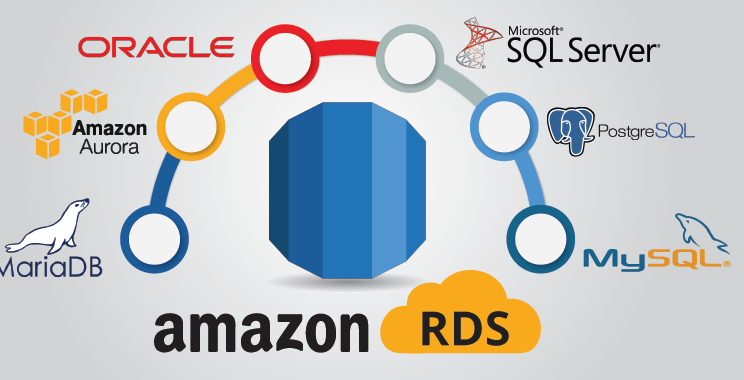
\includegraphics[width=\textwidth]{rds.png}
    \caption{Relational Database Service}{\cite{36}}
    \label{fig:rds}
\end{figure}

\par The pricing of Amazon Relational Database Service is based on usage.
The cost is dependent on various parameters such as instance hours, the number of input and output transactions, storage capacity, size of backup storage, or amount of Internet data transfer.
Different applications use different instance types.
The database instance is a fundamental element of the
Amazon RDS. A database engine works in each database instance with function parameters and specific properties that determine and control the properties of the databases. Database instances can be created, configured, and deleted using the AWS CLI, AWS management console, or RDS API. Computing and storage and capacity, database engine, and other parameters such as backup, version and update settings, or master user access data must be specified for each database instance. Depending on the type of database engine the number of databases per instance varies for example, with Microsoft SQL Server, up to 100 databases are possible, Oracle allows one database per instance, MySQL, MariaDB, Amazon Aurora, and PostgreSQL have no software limitations on the maximum number of databases \cite{37}.

\par Security of Amazon RDS and the stored or transmitted data is implemented at various levels.
AWS IAM controls which application or which user has access to which database resources and functions.
Depending on the requirements, groups and users are created and specific access rights are assigned.
Database instances are in a protected Amazon \gls{vpc}.
The access to the traffic that flows in and out of a DB instance is controlled by the VPC security groups.
The access to the DB instance is turned off by default.
In order to improvise security, access to the DB instance can be restricted to a specific IP address range, port or security group.
This can be achieved by specifying rules in a security group.
A total of 20 rules can be specified in a security group.
Once the rules are configured, every DB instance associated with that security group follows the same rules.
VPC security groups define which devices or instances can connect to a database instance.
The connections are encrypted and secured using Transport Layer Security (TLS) / Secure Sockets Layer (SSL) or IPsec VPNs. Amazon RDS firewall settings control network access. Database data at rest can be encrypted and database events can be logged \cite{71}.

\textbf{Features of RDS Instances}
\begin{itemize}
    \item \textbf{Amazon RDS Resources Encryption:} Data that is encrypted includes the underlying storage for DB instances, its automated backups, snapshots, and read replicas.
    The industry standard AES-256 encryption algorithm is used by the Amazon RDS encrypted DB instances to encrypt the data that is stored on the DB instances.
    After the data encryption is enabled, with minimal impact on the performance Amazon RDS handles decryption of data and authentication of access transparently.
    There is no modification needed in the database client to use encryption \cite{37}.
\end{itemize}
\begin{itemize}
    \item \textbf{Automatic backups:} Amazon RDS provisions creation and saving automatic backups of RDS DB instance.
    It
    provides users the capability choose a retention period and restore databases to any time during that period.
    Users can also take snapshots of instances manually and these snapshots remains until manually deleted \cite{37}.
\end{itemize}
\begin{itemize}
    \item \textbf{Replication:} Amazon RDS uses built-in
    replication functionality of Microsoft SQL Server, Oracle, MariaDB, and PostgreSQL DB engines to create a read replica, which is a special type of DB instance, from the source DB instance.
    A read replica represents a copy of the actual instance that reflects changes to the actual in almost real time and under normal circumstances.
    Figure \ref{fig:readreplicasworking} shows a pictorial view of the working of read replica \cite{37}.
\end{itemize}
\begin{figure}
    \centering
    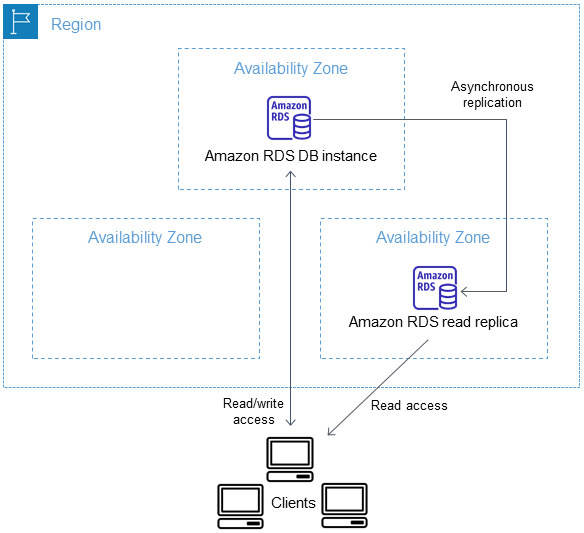
\includegraphics[width=\textwidth]{readreplicasworking.png}
    \caption{AWS RDS DB Instance Replication}{\cite{38}}
    \label{fig:readreplicasworking}
\end{figure}
\begin{itemize}
    \item \textbf{Performance metrics and monitoring:} Amazon provides CloudWatch service that enables managed
    monitoring.
    Amazon CloudWatch make it possible for the users to
    view capacity and I/O metrics \cite{37}.
\end{itemize}



\textbf{Amazon Simple Storage Service (S3)}

\par Amazon \gls{s3} is a high-speed, scalable, object
storage
service
in cloud that offers data availability, security and high performance.
Amazon S3 enables backup and archiving of data and
applications in AWS. It can store any type of object,
which allows uses like storage for Internet applications, data archives, backups, disaster recovery, hybrid cloud storage, IoT devices, and data lakes for analytics \cite{39}.

\par Storing, organizing, and retrieving data in Amazon S3 primarily focuses on two key components: objects and buckets that work together to create the storage system.
The Amazon S3 object storage data model is a flat structure.
The bucket stores the objects, once the bucket is created.
There is no real hierarchy of sub buckets or subfolders but a logical hierarchy can be inferred using key name prefixes and delimiters.
The objects are data files which include photos,
documents, and videos. Each object in the S3 environment
is identified by a unique key that differentiates it from other objects. The buckets serve as the fundamental storage containers for objects. While creating the bucket AWS provides users the ability to choose the AWS region. Even though a bucket is associated with a specified region, the name of the bucket acts as a global identifier, thus the name of the bucket must be unique among all the buckets across the world. The figure \ref{fig:s3} show Amazon S3, buckets and objects \cite{40}.

\par Amazon S3 offers features to organize and manage data to operate cost-effectively, support specific use cases,
increase security, and meet compliance requirements.
With S3 Versioning, it is possible to keep multiple variants of an object in the same bucket.
S3 Versioning helps to preserve, retrieve, and restore every version of every object stored in the buckets.
Amazon S3 generates a unique version ID once the S3 versioning in a bucket is enabled for each object added to the bucket.
Objects that already existed in the bucket at the time
versioning is enabled, such objects get assigned with a
version ID of \textit{null}. If an object is modified, such as \textit{CopyObject} and \textit{PutObject}, the new objects get a unique version ID \cite{41}.

\begin{figure}
    \centering
    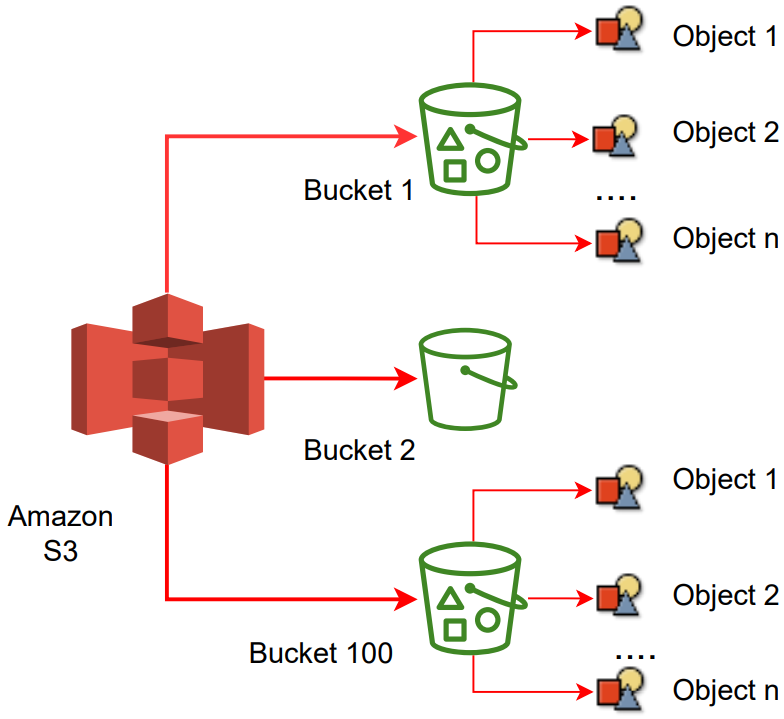
\includegraphics[width=\textwidth]{s3.png}
    \caption{Amazon Simple Storage Service}{\cite{42}}
    \label{fig:s3}
\end{figure}

\par Access to S3 objects is managed using the Identity
and access management service (IAM), bucket policies, S3
access points, and \gls{acl}.
With the Identity and access management service (IAM), it is possible to manage the access on the user or group level, it is also possible to delegate permissions to the S3 bucket to other AWS customer accounts.
To grant access permissions to the bucket and the objects, a resource-based AWS IAM policy called a bucket policy is used.
Associating a policy with a bucket can only be done by
the bucket owner.
JSON-based access policy language is used to create Bucket policies.
The bucket policies can be used to add or deny permissions for the objects in a bucket.
Amazon S3 Access Points describe how data can be accessed using that endpoint.
To perform S3 object operations such as
\textit{PutObject} and \textit{GetObject}, access points are
attached to buckets are used, .
Each S3 access point has its own access point policy.
To authorized users for individual objects and buckets, ACLs grants read and write permissions.
ACL are attached as a sub resource to each bucket and objects.
The ACL defines which AWS groups or accounts are granted access and the type of access to which the access is granted.
The Block Public Access feature in Amazon S3 provides settings for accounts, access points, and buckets to help user manage public access to resources.
By default, public access is not allowed on access
points, new buckets, and objects, however, users can
modify the access point policies, bucket policies, or object-related permissions to allow public access \cite{43}.

\par There are four settings provided by S3 Block Public
Access.
These settings can be applied in combination to individual buckets, access points, or entire AWS accounts. Upon applying a setting to an account, the setting is applied to all the access points and buckets that are owned by that account. Similarly, if the setting is applied to a bucket, it
applies to all access points associated with that bucket. Table \ref{tab:blockpublicaccesssettings} highlights
different settings for blocking public access \cite{23}.



\begin{longtable}{|p{5cm}|p{11.4cm}|}
    \hline
    \textbf{Name} & \textbf{Description} \\
    \hline
    \textit{BlockPublicAcls} & When BlockPublicAcls is set to TRUE the following behavior are seen:
    \begin{itemize}
        \item If the specified access control list (ACL) is public, PUT Bucket acl and PUT Object acl calls fail.
    \end{itemize}

    \begin{itemize}
        \item If the request includes a public ACL, PUT Object calls fail.
    \end{itemize}

    \begin{itemize}
        \item On applying this setting to the AWS account, then PUT bucket call fails in a situation where public ACL is included in the request.
    \end{itemize}
    \par When BlockPublicAcls is set to TRUE, the above specified operations fail, however, existing policies and ACLs for buckets and objects are not modified. This setting enables protecting against public access while allowing to audit, refine, or otherwise alter the existing policies and ACLs for buckets and objects \cite{44}.
    \\
    \hline
    \textit{IgnorePublicAcls} & Setting IgnorePublicAcls to TRUE causes Amazon S3 to ignore all public ACLs on a bucket and any objects it contains.
    This ensures the public access granted by ACLs will be blocked, while the PUT object calls that include a public ACL will still be allowed.
    The persistence of any existing ACLs does not get affected by enabling IgnorePublicAcls, and also it doesn't prevent new public ACLs from being set. \cite{44}.  \\
    \hline
    \textit{BlockPublicPolicy} & When BlockPublicPolicy is set to TRUE for a bucket, Amazon S3 rejects calls to PUT Bucket policy if the BlockPublicPolicy allows public access. When BlockPublicPolicy is set to TRUE for an access point, Amazon S3 rejects calls to PUT access point policy and PUT Bucket policy that are made through the access point if BlockPublicPolicy (for either the access point or the underlying bucket) is public \cite{44}.  \\
    \hline
    \textit{RestrictPublicBuckets} & The access to a bucket or access point with a public policy to authorized users and principals within the bucket owner's account will be restricted on setting RestrictPublicBuckets to TRUE.
    All cross account access to the bucket or access point are blocked by RestrictPublicBuckets, while it will still be possible for the users within the account to manage the bucket or access point \cite{44}.  \\
    \hline
    \caption{Block public access settings}
    \label{tab:blockpublicaccesssettings}
\end{longtable}

\textbf{Lambda:}
\par AWS Lambda is a serverless computing service that lets the users run code without provisioning or managing servers.
Lambda runs the code on a highly available compute
infrastructure and performs all the administrative tasks
of the compute resources, including capacity provisioning, code monitoring, server and operating system maintenance, automatic scaling, and logging \cite{45}.

\par With Lambda, it is possible to run code for virtually any type of application or backend service by supplying the code in one of the languages that Lambda supports.
The code is organized into Lambda functions.
Lambda runs the function only when needed and scales automatically, from a few requests per day to thousands per second.
Lambda functions are invoked using the Lambda API or as a response to an event from other AWS services.
There is no charge when the code is not running, users
pay only for the compute time that Lambda consumes
\cite{46}.

\par Lambda is an ideal compute service for many application scenarios, as long as the user can run the application code using the Lambda standard runtime environment and within the resources that Lambda provides.
When using Lambda, users are responsible only for their code.
Lambda manages the compute fleet of resources that offers a balance of memory, CPU, network, and other resources to run the code.
Because these resources are managed by Lambda, users cannot customize the operating system or login to compute instances on provided runtimes.
Lambda performs administrative and operational activities on behalf of users, including managing capacity, monitoring, and logging the Lambda functions.
AWS manages the entire infrastructure layer of AWS Lambda
and thus saves user time on operational tasks. AWS Lambda
provides a distinctive architectural property by enabling many instances of the same function, or of different functions from the same AWS account, to execute concurrently. This makes AWS Lambda a good fit for deploying highly scalable cloud computing solutions \cite{46}.

\par AWS Lambda invokes the function in an execution environment.
The execution environment provides an isolated and secure runtime environment and manages the resources required to run the function.
The support for any external extensions associated with the function or function's runtime is provided by execution environment.
The runtime of function and each external extension are
processes that run within the execution environment
\cite{46}.

\par The following phases are included in the execution
environment:
\begin{itemize}
    \item \textbf{Init phase}: In the init phase, Lambda unfreezes or creates an execution environment with the configured
    resources, downloads the code for the function and all layers, initializes the runtime, initializes any
    extensions, and then runs the function’s
    initialization code \cite{46}.
\end{itemize}
\begin{itemize}
    \item \textbf{Invoke phase}: During this phase, Lambda invokes the function handler. After the function runs to
    completion, Lambda prepares to handle another
    function invocation \cite{46}.
\end{itemize}
\begin{itemize}
    \item \textbf{Shutdown phase}: The shutdown phase is triggered if the Lambda function does not receive any invocations
    for a period of time.
    During the shutdown  phase, the runtime is shutdown
    by Lambda, it send an alert to each extension for
    stopping cleanly, and finally removed the environment \cite{46}.
\end{itemize}


\section{Security Framework}

\begin{figure}
    \centering
    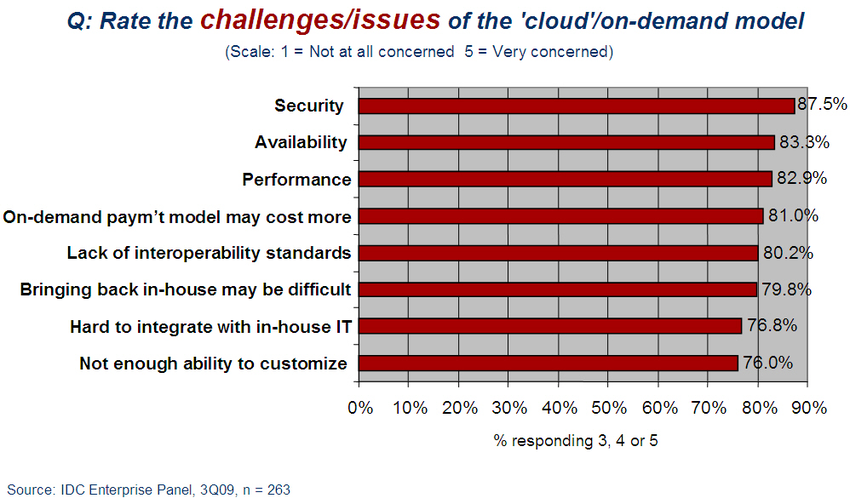
\includegraphics[width=\textwidth]{securitychallenges.png}
    \caption{Results of IDC ranking security
    challenges}{\cite{47}}
    \label{fig:securitychallenges}
\end{figure}

\par \gls{csp} leverage
virtualization technologies combined with self-service capabilities for computing resources via the Internet.
In these service provider environments, in order to maximize the efficiencies of virtualization, virtual machines must be located on the same physical server.
Based on a survey conducted by IDC as seen in the figure \ref{fig:securitychallenges}, of 263 IT executives and their line-of-business, security is ranked first as the greatest issue or challenge of cloud computing \cite{47}.

\par Information security management encompasses many areas from encryption and perimeter protection to application security and disaster recovery.
Security in IT is made more complex by compliance regulations, such as PCI, DSS, HIPAA, Sarbanes-Oxley, and global standards, such as GDPR. While most compliance experts and CEOs understand the value of cybersecurity measures, IT standards and security frameworks can make safeguarding organizations feel daunting.
Knowledge of standards, regulations, and frameworks is
essential for all infosec and cybersecurity professionals
\cite{48}.

\par A security framework is a compilation of international cybersecurity procedures and policies and state-mandated for maintaining and establishing security controls to protect critical infrastructure from cybersecurity risks.
These security frameworks are a blueprint for reducing vulnerabilities and managing risk by helping IT security professionals keep their organizations compliant and insulated from cyber threats.
The frameworks are used by Information security professionals to prioritize and define the tasks required to manage enterprise security.
It is possible for organizations to customize frameworks
to solve specific information security problems, such as
industry-specific requirements or different regulatory compliance goals \cite{48}.

\subsection{Prowler}

\par This research aims to introduce a framework called Prowler that can identify the security vulnerabilities or misconfigurations that exist in AWS accounts.
The thesis work focuses on the most popular AWS services,
IAM,
EC2, Lambda, S3, and RDS.
The introduced framework indicates to which security vulnerabilities the application is vulnerable and which security issues must be addressed to resolve the security vulnerability.
Prowler contains a set of controls, mapped against known security vulnerabilities, which can determine whether a given AWS cloud setup is vulnerable to these security vulnerabilities.
It aims to provide more in-depth security for AWS RDS,
EC2, IAM, S3, and Lambda resources and protects them
against security vulnerabilities.\\

\hfill \break
\par Prowler is an open-source AWS Security Best Practices Assessment, Hardening, Auditing, and Forensics Readiness command line tool.
Prowler scans the AWS account to check for potential security vulnerabilities, overly permissive Identity and Access Management (IAM) permissions, and best practice violations.
Using Prowler, it is possible to evaluate the AWS
security specifically against the CIS AWS Foundations
Benchmark and has more than 190 additional checks related
to \gls{hippa}, \gls{gdpr}, \gls{pci-dss},
ISO-27001, FFIEC, SOC2,
and
others \cite{49}.
Prowler provides more than 240 checks covering security best practices across all AWS regions and related to AWS services such as Amazon CloudFront, Amazon Redshift, Amazon ElasticCache, Amazon API Gateway, etc.
It helps organizations implement practices that ensure
having proper security measures in place and a secure
environment.
Prowler supports the generation of assessment reports in multiple formats such as JSON, CSV, HTML, JUnit, or JSON ASFF Security Hub.
The colorful or monochrome report enhances the user’s visibility.
Prowler also supports running a specific check or groups or creating your own.
When running the Prowler assessment, prowler supports
checking multiple AWS accounts in Parallel or
sequentially \cite{50}.\\
\hfill \break
\par Prowler is written in bash, and it uses AWS-CLI
underneath.
It works with multiple operating systems such
as macOS, Linux, or Windows with Cygwin or virtualization.
To use Prowler, though, an EC2 instance with the necessary security permissions can be provisioned, Fargate or any other container, CloudShell, Codebuild, and Cloud9.
Prowler can also be deployed directly in AWS using the AWS
CLI and other components such as Python pip,
detect-secrets, an open-source tool used to detect secrets by running scans, and jq , a flexible and lightweight command-line JSON processor already installed.
Detect-secrets is  \cite{50}.
\hfill \break
\begin{figure}
    \centering
    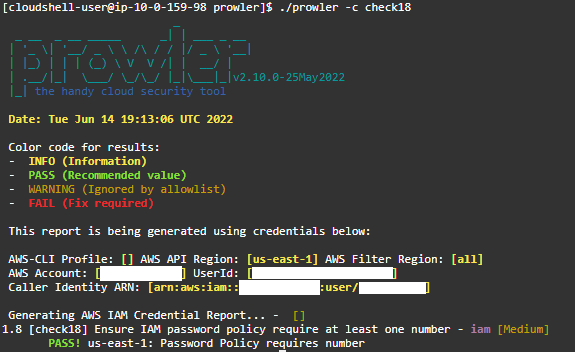
\includegraphics[width=\textwidth]{prowlercheckpass.png}
    \caption{Check execution in Prowler}
    \label{fig:prowlercheckexecution}
\end{figure}

\par After installing the required tools and packages
successfully, the AWS environment need be configured with
a valid Access Key and Region or by declaring the AWS
variables.
This can be done by running the command \textit{aws configure}.
In order to run all the Prowler checks, managed policies
\textit{SecurityAudit} and \textit{ViewOnlyAccess} must
be added to the user \cite{47}.



Prowler can then be installed directly by cloning the
code for the source repository \cite{48} using the
command \textit{git clone https://github.com/prowler-cloud/prowler} and does not require any additional setup afterward.
Once the source code is available, the assessment of security vulnerability using Prowler is performed by executing the command \textit{./prowler}.
Figure \ref{fig:prowlercheckexecution} shows the execution of the check using Prowler.
When the command is run, Prowler authenticates the configured environment variable.
Upon successful authentication, the checks are run over all the AWS regions.
To limit the assessment to a custom profile and region, the command \textit{./prowler -p custom-profile -r us-east-1} is used.
Prowler also enables assessing a single security vulnerability by running the command \textit{./prowler -c check78}.
The check78 is a check id, this check ensures there are no Public Accessible RDS instances (verifies publicly accessible RDS instances).
Table \ref{tab:prowlerextra} shows the execution result
of the assessment performed using Prowler \cite{48}.
\begin{table}[h!]
    \begin{center}
        \caption{Prowler check execution result}
        \label{tab:prowlerextra}
        \begin{tabular}{|p{1.4cm}|p{1.7cm}|p{1.5cm}|p{4.0cm}|p{5.0cm}|}
            \hline
            \textbf{Result} & \textbf{Severity} & \textbf{CheckID} & \textbf{Check Title} & \textbf{Check Output}\\
            \hline
            Pass & Critical & 7.8 & [extra78] Ensure there are no Public Accessible RDS instances &
            No Publicly Accessible RDS instances found\\
            \hline
        \end{tabular}
    \end{center}
\end{table}

\par If the user wants to save the assessment report for later analysis, Prowler enables saving the result in different formats such as CSV, JSON, Html, etc.
The command to generate the assessment report in CSV
format is
\textit{./prowler
-M csv} \cite{49}.

\begin{figure}
    \centering
    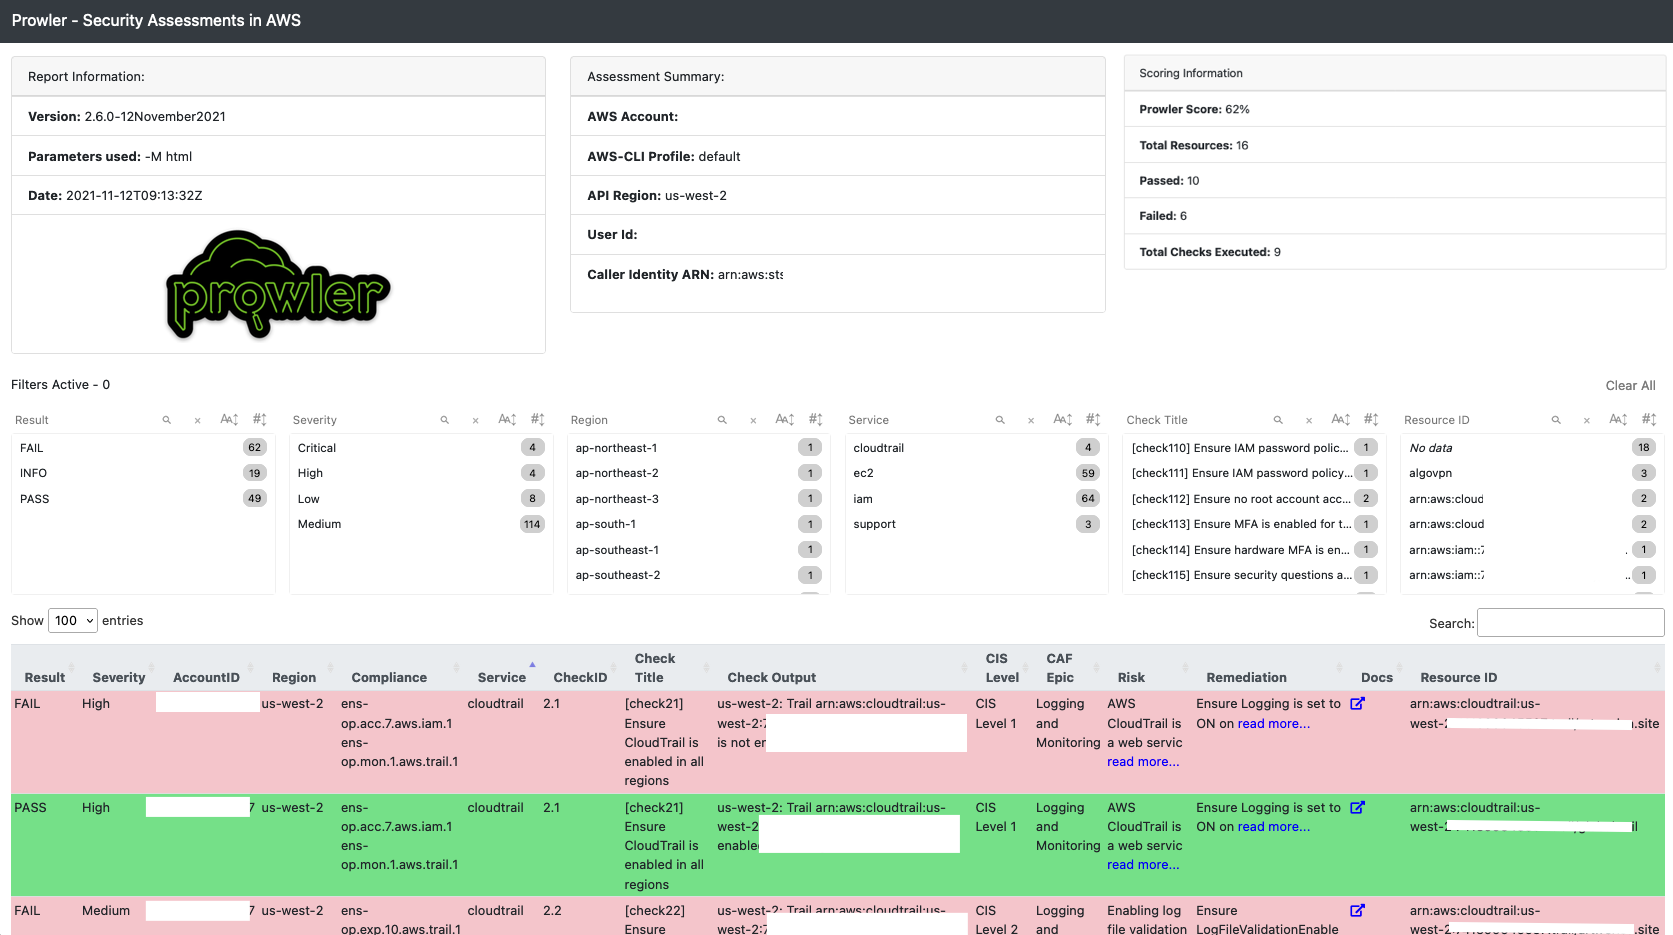
\includegraphics[width=\textwidth]{prowlerassessmentreport.png}
    \caption{Assessment report in Prowler}
    \label{fig:assessmentreport}
\end{figure}

The figure \ref{fig:assessmentreport} shows the
assessment report generated after the assessment of AWS
account using Prowler.
%! Author = vsharma
%! Date = 25.09.2022
% !TeX spellcheck = en_EN

\chapter{Problem Statement}

\par Due to the increase in the rate of cybercrime attempts, growing amounts of data, digital business models, insider threats, human error, etc., security remains a very important topic for companies and their customers \cite{40}.
 These crimes basically refer to the misuse of information and technology for illegal and unauthorized access to resources as seen in figure \ref{fig:securityAttack}.
 Despite the development of offensive tools and
capabilities, the number of security attacks has not been
fully addressed on a truly global \cite{50}.
 Based on the different research work and literature, this chapter highlights various security vulnerabilities in different AWS services.

\begin{figure}
    \centering
    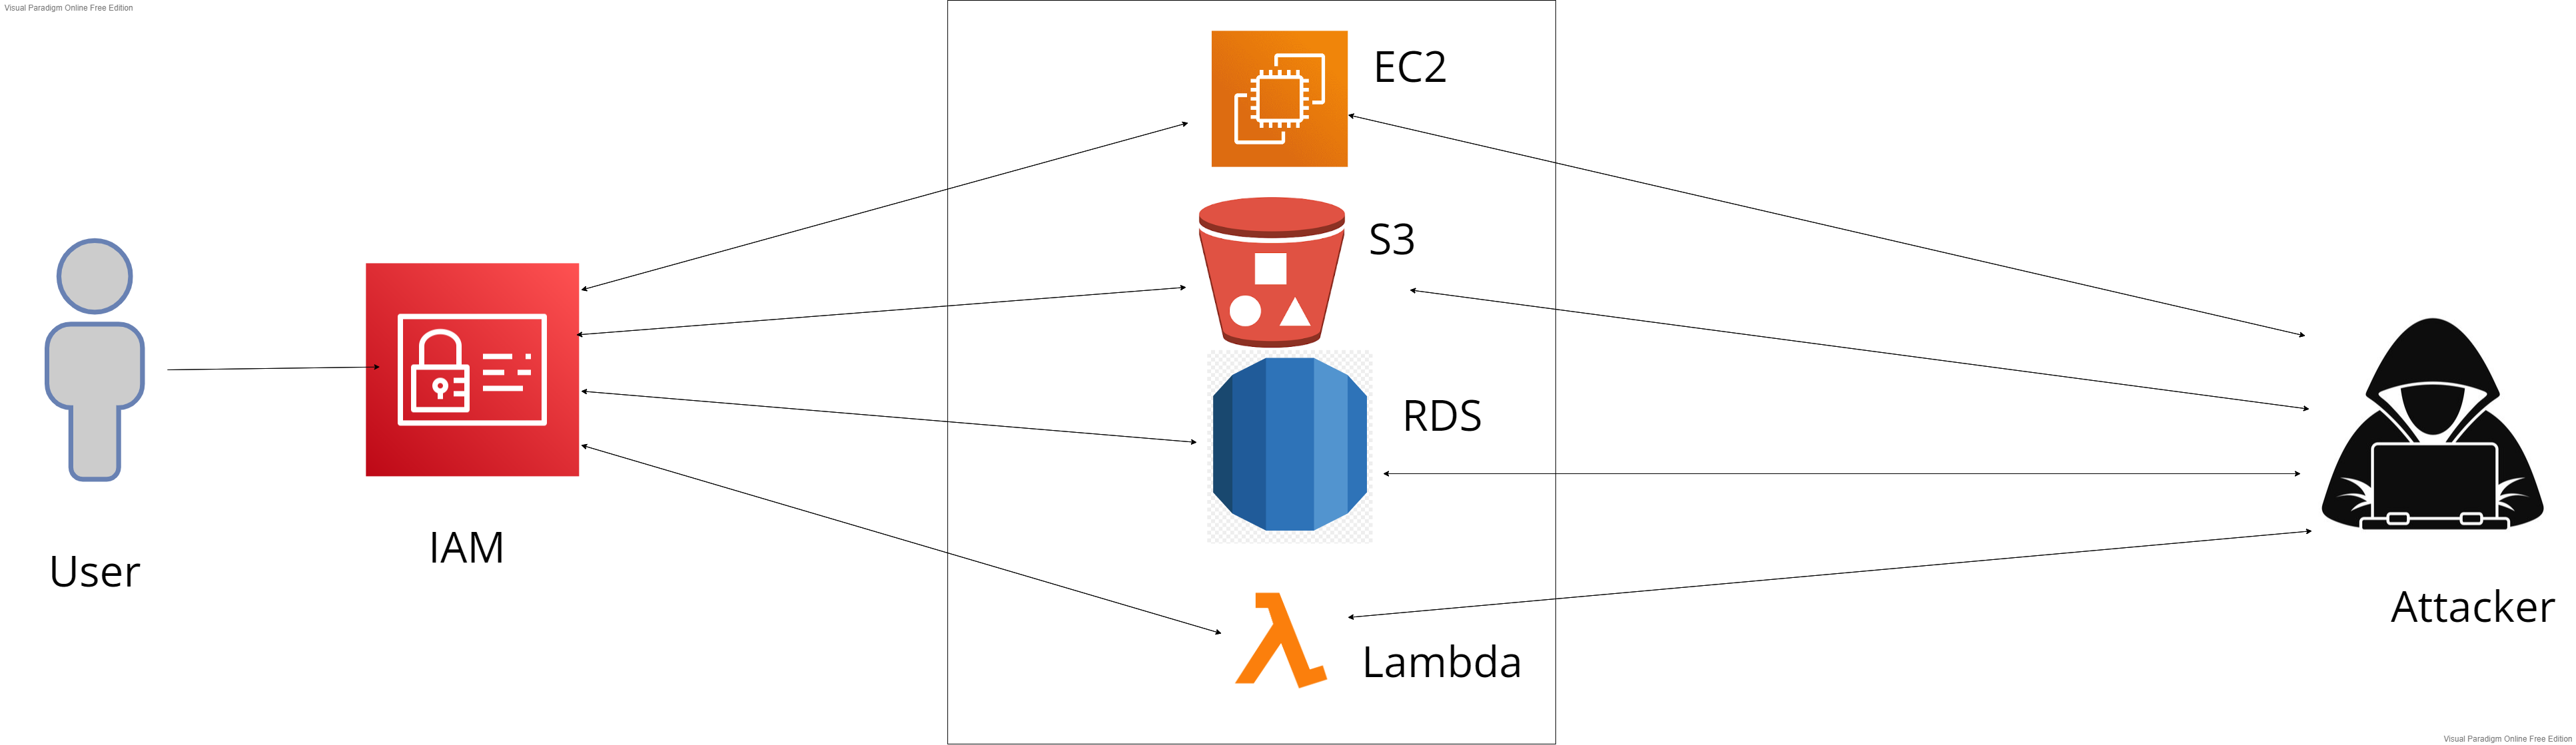
\includegraphics[width=\textwidth]{securityAttack.png}
    \caption{AWS Services Security vulnerabilities}
    \label{fig:securityAttack}
\end{figure}

\section{Identification of Security Vulnerabilities}

\par This section lists the several security vulnerabilities and misconfigurations identified in five AWS services
based on literature, the \gls{owasp} vulnerability list
\cite{51},
\gls{cisa}
\cite{52}, \gls{idc} \cite{53}.


\begin{itemize}
    \item \textbf{Excessive privileges:} Additional Permissive Policies granted to the users beyond what they need.
    This type
    of security vulnerability occurs when the users are
    granted more access than required for their job
    \cite{54}. It is
    sometimes hard to keep up with every user’s permission as every application and system has its own application
    model \cite{55}.
\end{itemize}

\begin{itemize}
    \item \textbf{Insider threat:} Insider threat refers to a person who has the required access rights to an
    information system and misuses his privileges.
    In the last years, it has been experienced that most companies have outsourced their IT infrastructure.
    Outsourcing affects the organization’s risk profile inevitably.
    Characterization of such attackers is not straightforward.
    For example, consider an employee who has been fired.
    In order to take revenge on his former employer, the
    employee plans an attack.
    Even though the employee's access rights should have been revoked, and the employee is not considered a
    legitimate user anymore, if the employee still has
    access to the infrastructure using a backdoor the employee has previously installed, this employee is still considered an insider threat \cite{56}.

    Insider threats can be classified into two contexts:
    \begin{itemize}
        \item \textbf{Cloud provider:} Where the insider
        is an employee working for the cloud provider i.e
        ., a cloud provider has a malicious system
        administrator working for them.
        The insider can use the authorized access
        rights to access sensitive information \cite{56}.
    \end{itemize}
    \begin{itemize}
        \item \textbf{Cloud outsourced:} The insider is an employee of an organization, which has outsourced its
        infrastructure to the cloud \cite{56}.
    \end{itemize}
\end{itemize}

\begin{itemize}
    \item \textbf{Misconfiguration:} Management of configuration is the most important part of network management.
    Bad or Incorrect configuration can have dramatic effects on the security and safety of users, applications, and the overall system. Most data breaches and cyber-attacks in cloud infrastructure are due to misconfiguration vulnerabilities and human errors \cite{44}.

    Various misconfiguration vulnerabilities exist in cloud environments.
    A few examples of misconfiguration are: Not
    using MFA, reusing passwords, using the Root account’s access keys, weaker password policy, misconfiguration of S3
    buckets,  misconfiguration of RDS
    instances, etc \cite{55}.
\end{itemize}

\begin{itemize}
    \item \textbf{Instances created from Malicious AMI:} With the organizations moving their infrastructure, data,
    and workload to the cloud, it is important that the
    \gls{ami}
    from the AWS Marketplace that are
    used in creating the EC2 instance are safe. AMI is used to create virtual servers on the AWS environment.
    Malicious AMI pose significant risks as the embedded code can include ransomware, crypto miners, malware, and so
    on {57}.

    An AMI basically includes the following:
    \begin{itemize}
        \item A template (typically an operating system, e.g., Amazon Linux, Ubuntu, etc., an application server and applications) for the root volume of the instance.
    \end{itemize}
    \begin{itemize}
        \item Launch permissions ensuring the authorized accounts can use the AMI to launch instances.
    \end{itemize}
    An instance was investigated by Summit Route in 2018
    where a Monero miner malware was embedded in an
    Ubuntu AMI \cite{57}.
    Similarly, in 2020, researchers at Mitiga during the assessment of an organization’s AWS environment found an
    active crypto miner on an EC2 instance, later during the review, it was revealed that the crypto miner was
    embedded in the AMI used by the organization \cite{58}.
\end{itemize}

\begin{itemize}
    \item \textbf{User data public exposure:} Exposure of user data is a critical vulnerability in cloud environments.
    Instance user data is a metadata field allowing custom code to run after the instance is launched.
    This metadata
    contains code that is exposed to any entity which has access to EC2, even the most basic access to EC2 for
    example, read-only configurations \cite{48}.

    While user data is an efficient way to automate the launch of scripts at instance launch, EC2 user data is a
    significant place where secrets can be unnecessarily exposed.
    For example, if password need to be used as part of
    a script we might be tempted to store it as plaintext in the script that we input to the user data.
    If the secrets are stored as plain text, then any user with ec2:DescribeInstanceAttribute permission will be able to view the secrets \cite{59}.

    Another example is when an instance pulls an application from a private Git repository.
    As the repository is
    private it can be accessed using the SSH key.
    Often this key is hard-coded in the user data.
    Attacker can get
    access to the private source code of the application if the attacker gets access to the instance user data.
    The attacker can access the user data if he is able to query the IMDS from the EC2 instance, e.g using an SSRF
    vulnerability.
    The attacker can read the user data directly from the
    AWS \gls{api} ,if the attacker has valid AWS
    credentials with the ec2:DescribeInstanceAttribute
    IAM permission \cite{60}.
\end{itemize}

\begin{itemize}
    \item \textbf{\gls{ssrf}:} \gls{ssrf} is a web security
    vulnerability allowing an attacker to make requests to an unintended location through the server-side application.

    SSRF tricks the web application to make an HTTP request on behalf of the attacker to a URL. This allows the
    attacker to get access to sensitive data or information that are exposed directly, or the attacker does not have
    access to, for example, AWS metadata, external web services, or other web applications based within the
    organization’s infrastructure.
    Sometimes is it also possible for the attacker to perform arbitrary command
    execution \cite{61}.
    SSRF is mostly encountered \cite{62}:
    \begin{itemize}
        \item If an attribute enables file generation methodology for example PDF generation.
    \end{itemize}
    \begin{itemize}
        \item If there is a file upload such as uploading the scanned images, documents, files, etc.
    \end{itemize}
\end{itemize}

\begin{itemize}
    \item \textbf{Denial of Wallet:} The Denial of Wallet is a form of security vulnerability unique to serverless
    computing,
    that results in financial exhaustion of the victim in the form of inflated usage bills.
    The execution costs are
    primarily increased via excessive function run time, additional resource consumption, and invocation count.
    This
    is usually achieved by exploiting the massive capability for scaling.
    The platform will be capable of handling
    such increased load but will incur costs for doing so
    \cite{63} \cite{64} \cite{65}.
\end{itemize}

\begin{itemize}
    \item \textbf{Public RDS Database instance:} Amazon RDS, a web service that enables setting up and scaling
    relational databases in the cloud for the web applications.
    Minimizing data loss and security risks can be
    ensured by checking the database’s instance for
    restricting unauthorized access and public
    accessibility \cite{66}.

    The RDS instance is within a \gls{vpc}.
    The default VPC consists of three subnets used to 
    isolate resources inside the VPC. A subnet within a 
    VPC is a segment of a VPC's IP address range used to 
    group DB instances based on security and operational 
    needs \cite{67}.

    Subnets are segments of a VPC's IP address range that users designate to group the resources based on operational and security needs.
    A collection of subnets created by the user and is then designated for the DB instances is called a DB subnet group.
    Each DB subnet group has subnets in at least two Availability Zones in a given AWS Region.
    When a DB instance is created in a VPC, a DB subnet group for the DB instance is chosen by the user.
    From the DB subnet group, Amazon RDS chooses an IP address within that subnet and a subnet to associate with the DB instance.
    The Availability Zone that contains the subnet is
    used by the DB. The subnets in a DB subnet group can
    be either private or public and it depends on the
    configuration that users set for their network ACLs
    and routing tables. For a DB instance to be publicly accessible, all the subnets in its DB subnet group must be public. If a subnet changes from public to private, it can affect DB instance availability \cite{67}. If an AWS account is Provisioned with public-facing RDS database instances it allows unauthorized access for anyone who establishes a connection to the database, thus introducing security risks \cite{68}.
\end{itemize}

\begin{itemize}
    \item \textbf{AWS classic resources:} AWS EC2-Classic is Amazon's original version of EC2,
    it started with one instance type, security groups, and the venerable US East (N. Virginia) Region.
    The EC2-Classic model of the network was flat, it had public IP addresses that were assigned at launch time.
    AWS classic resources run on the shared environment along with infrastructure owned by other AWS customers for
    example ClassicLink unlike a virtual private cloud
    (VPC) which is a dedicated virtual space for your Amazon Web Services account isolating from the rest of the virtual networks in the AWS cloud \cite{69}.
\end{itemize}

\begin{itemize}
    \item \textbf{Default data retention:} Amazon RDS provides a feature to create and save automated backups of your DB
    instance.
    RDS backs up the entire DB instance by creating a storage volume snapshot of the DB instance.
    This
    backup is saved according to the retention period specified.
    AWS has a default RDS backup retention for the
    cluster as 1 day which might be insufficient, hence backup retention should be set to a period that
    is within the balance and budget \cite{36} \cite{38}.
\end{itemize}

\begin{itemize}
    \item \textbf{Data Event Injection:} This kind of security vulnerability occurs due to bad coding practices such
    as bad
    deserialization of user input or using JavaScript \textit{eval ()} function.
    The Data event injection is the
    number
    one
    attack in the OWASP list of Serverless top 10
    security vulnerabilities \cite{68}.
\end{itemize}

\begin{itemize}
    \item \textbf{Insecure Management of Secrets:} \par Secrets management refers to the methods and tools for managing digital authentication credentials, such as passwords, tokens, and APIs keys for use in applications, privileged accounts, services, and other sensitive parts of the IT ecosystem.
    The terms secrets management and secrets are more commonly referred in IT with regard to DevOps processes, environments, and tools.
    \gls{devops} is a combination of a cultural philosophy,
    practices, tools, and mindsets enabling organizations to deliver sofware and applications reliably and faster.
    This show how DevOps is gaining more popularity and considered as a go-to model for rapid application delivery.
    When the product deadline is nearing, programmers
    often feel pressurized to meet the demands and in
    their haste leave sensitive pieces of code embedded in files, code, and applications. This may result in compromising organization’s security, for example, database credentials, IAM permissions, API keys, etc \cite{70}.

    Unlike insider threats, where the attacker intentionally misuses his privilege due to a personal grudge or some
    other issue, the secrets are sometimes hardcoded
    within the source code in plain text littered throughout configuration management tools and configuration files.
    Due to all these issues, there is a increasing  need
    for the organizations to centralize the auditing,
    storage, provisioning, rotation, and management of secrets in order to restrict the access to secrets and prevent thesecrets from compromising the organisation or leaking. There are services that share the same secrets, thus making identifying the source of compromise or leak challenging \cite{70}.
\end{itemize}

\begin{itemize}
    \item \textbf{Poisoning the Well:} Organizations usually rely on third parties for their business.
    Some examples
    in the
    digital world are libraries, and version control systems.
    It is important that
    these third parties are fully trusted when dealing with confidential data.
    Usage of third-party libraries is
    commonly practiced amongst developers within their codes.
    This makes it easy to re-use an already developed
    functionality either by himself or others.
    Attacker injects a malware in the libraries and wait for the version to be used by the developer in his code.
    \cite{71}.

    Lambda does not allow installating external libraries during the runtime, thus they must be shipped with Lambda function.
    This leads to the risk of using an outdated version of libraries as one would need to update the package and re-upload it to Lambda.
    In case a vulnerability is found inside a library and a patch is released, this might not be installed by the
    user who does not have a proper patching policy, thus
    leaving them vulnerable for a longer period \cite{72}.

    Although libraries can be susceptible to poisoning, it is not very likely this attack will be executed. If a Lambda function uses an out-of-date library, an attacker would still require access to the script or the input data triggering the function. As for impact, this depends on the permissions of the Lambda function. If the function has an over-permissive IAM Role, much can go wrong. If it is really strict and only allows minimal actions on minimal resources, the possibilities for an attacker are highly restricted. This makes the likelihood of the attack Neutral and the impact Medium. \cite{64}.
\end{itemize}

\par The above-listed security vulnerabilities associated with the different AWS services will be evaluated and assessed using security assessment tools in the next chapter.










%! Author = vsharma
%! Date = 25.09.2022
% !TeX spellcheck = en_EN

\chapter{Methodology}

\par AWS enables organizations to dynamically scale their applications and infrastructure.
However, due to the continuously addition of new services
and tools, new security challenges are
introduced.
Based on a report, 61 percent of \gls{smb} believe their
cloud
data is at risk and around 70 percent of organizations IT
leaders are concerned about how secure they are in the
cloud \cite{73}.
Although AWS is responsible for securing the infrastructure, it makes it clear to the users to ensure AWS services are properly configured according to best practices to avoid security vulnerabilities.

\par This research emphasizes identifying the efficiency of the open-source security assessment tool, Prowler.
To do so, different approaches are identified. This chapter explains the used approaches.


\section{Identification of Security vulnerabilities and Exploits}

\par AWS provides more than 100 services, and each of these services is vulnerable to security attacks.
These security vulnerabilities can be classified corresponding to each of the AWS services.
This research work is limited to 5 AWS services namely IAM, EC2, S3, RDS, and Lambda.
Columns 1 and 2 in table \ref{tab:classificationofsecurityvulnerabilities} lists the different security
vulnerabilities based on literatures, OWASP vulnerability
list \cite{51}, CISA \cite{52}, IDC \cite{53}.



\section{Prowlers Validation}

\par Prowler scans the AWS account to check for overly permissive IAM permissions, potential vulnerabilities, and best practice violations.
Prowler executes over 40 checks related to HIPAA and GDPR compliance and 49 checks against the CIS AWS Foundations Benchmark.
Prowler constantly checks the AWS accounts against the
CIS benchmarks for the AWS Cloud. Thus, ensuring that the
organization is operating in accordance with guidelines developed by industry consultants, audit and compliance organizations, software developers, operations specialists, security research organizations, government agencies, and legal experts \cite{74}.

\par To determine the efficiency of Prowler against security vulnerabilities two approaches are identified.
The first approach is a test-driven approach, it’s a
manual approach and the second approach uses an open-source application to evaluate the efficiency of Prowler against the identified security vulnerabilities \cite{47}.

\par In the end, another open-source assessment tool called ScoutSuite is used to perform the security assessment of the AWS account.
After the assessment using ScoutSuite finishes, the results are recorded.
The comparison between the assessment performed by the two open-source security
assessment tools are shown in the next chapter.

\subsection{Using Test Driven Approach}

\par A test case is a set of actions performed on a system to determine if it functions correctly. Test cases helps
in determining if different features within a system are performing as expected and to confirm that the system
satisfies all related standards, customer requirements and guidelines \cite{75}. This manual approach determines the
efficiency of Prowler against the identified security vulnerabilities listed in table \ref{tab:classificationofsecurityvulnerabilities}.

\par Prowler provides several checks to perform security assessments.
These checks help determine whether good practices are being followed to secure the set of resources. For each security assessment check in Prowler, we develop test cases to verify the positive and negative scenarios. In the end, the efficiency of Prowler is determined against the identified security vulnerabilities.

\subsubsection{Algorithm and Flowchart}

\begin{figure}
    \centering
    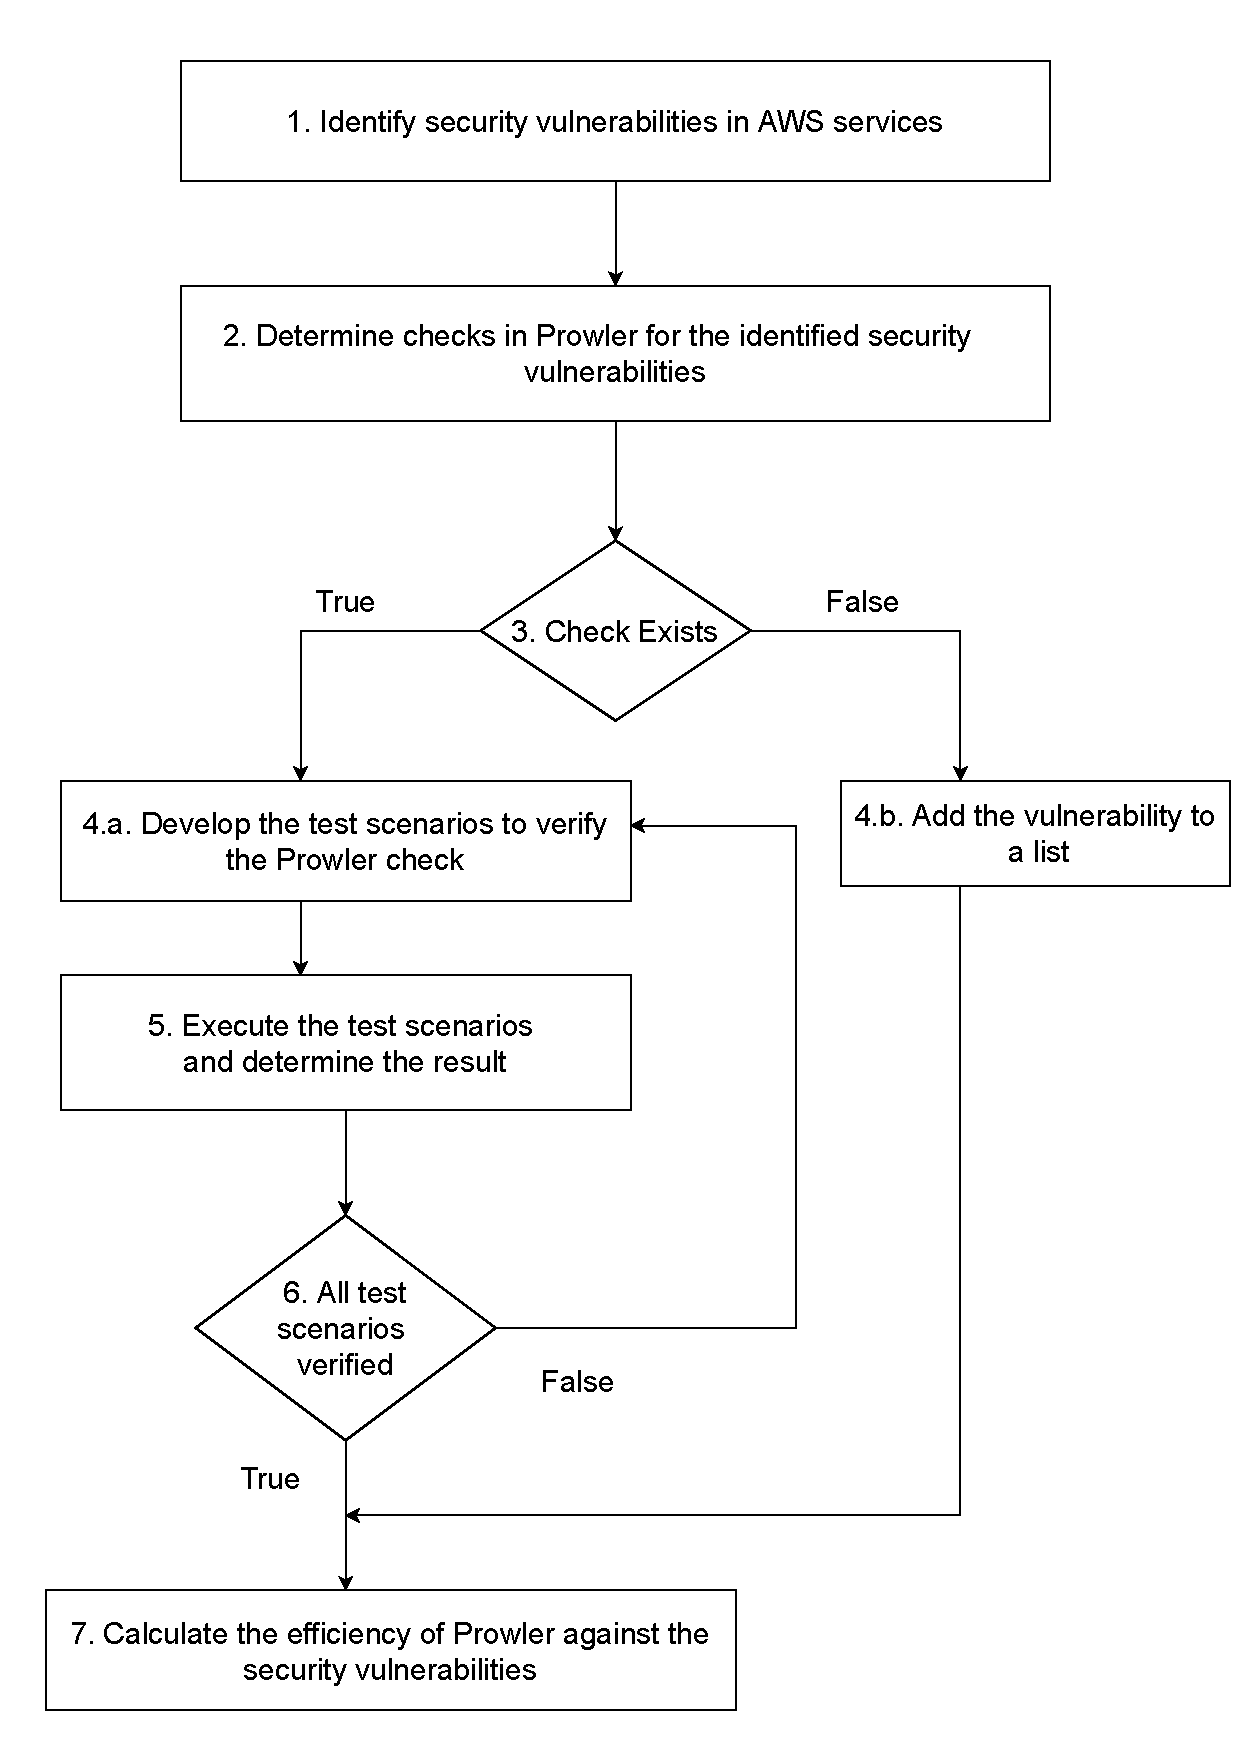
\includegraphics[width=\textwidth]{flowdiagram.pdf}
    \caption{Security vulnerability Assessment flow diagram}
    \label{fig:flowdiagram}
\end{figure}
\begin{itemize}
    \item As an initial step, the process starts by identifying the security vulnerabilities in the five AWS services.
    The different security vulnerabilities are identified
    based on literatures, OWASP vulnerability list
    \cite{51}, CISA \cite{52}, IDC \cite{53}.
    This is highlighted as Step 1 in the flow diagram \ref{fig:flowdiagram}.
\end{itemize}
\begin{itemize}
    \item After the identification of security vulnerabilities, the next step is to identify checks in Prowler that assesses the security vulnerabilities identified in step 1.
    This corresponds to steps 2 and 3 in the flow diagram \ref{fig:flowdiagram}.
\end{itemize}
\begin{itemize}
    \item For each check in Prowler develop the test scenarios in python and verify the test scenarios. The result of the test scenarios is noted. These are steps 4.a and 5 in the flow diagram. This process repeats until all the possible checks are verified successfully.
\end{itemize}
\begin{itemize}
    \item If a check does not exist in Prowler for the security vulnerability, add the security vulnerability in a separate list.
    Step 4.b in the flow diagram \ref{fig:flowdiagram} highlighted this process.
\end{itemize}
\begin{itemize}
    \item In the end, the efficiency of Prowler is calculated between the verified security vulnerabilities using the checks in Prowler and the security vulnerabilities identified initially in Step 1 of the flow diagram.
    This is represented as Step 7 in the flow diagram \ref{fig:flowdiagram}.
\end{itemize}


\par The test cases are developed for each check in Prowler.
As we see from the listing
4.1, the method check15\_require\_upper\_case\_characters() calls the test case methods
for positive and negative scenarios.
The positive scenario is verified using the method
check15\_require\_upper\_case\_characters\_true() and the negative test scenario is verified
using check15\_require\_upper\_case\_characters\_false().

\par Python boto3 \cite{76} library is used in the test
cases.
Boto3 is the Python SDK for AWS
that allows creating, updating, and deleting AWS resources directly from your Python
scripts.

\par As a first step, for each scenario the AWS resource
such as IAM, EC2, etc. are enabled using boto3 \cite{76}.
Upon enabling the resource, the method associated with the resource is determined and used to set the value on the argument, for example, RequireUppercaseCharacters is set to True in this case. After setting the required value on the argument, the check is executed. After the execution of the check finishes, the return code for the test scenario is determined. Once the return code is obtained, it is verified. Only after the verification is successful, the security vulnerability is added to the list of security vulnerabilities verified using prowler.


\lstset{frame=lines}
\lstset{caption={Test code implementation for Prowler assessment}}
\lstset{label={lst:code_check15}}
\lstset{basicstyle=\footnotesize\ttfamily}
\lstset{numberstyle=\tiny\color{cyan}}
\lstset{keywordstyle=\color{red}}
\lstset{identifierstyle=\color{blue}}
\lstset{stringstyle=\color{orange}}
\lstset{commentstyle=\itshape\color{purple!40!black}}
\lstset{
    numbers=left,
    firstnumber=1,
    numberfirstline=true,
    numberstyle=\tiny\color{green},
}

\begin{lstlisting}[language=Python]
	def check15_require_upper_case_characters_true(self):
            client = boto3.client('iam')
            client.update_account_password_policy(RequireUppercaseCharacters=True)
            response = subprocess.run(["./prowler", "-c", "check15"])
            return response.returncode
        def check15_require_upper_case_characters_false(self):
            client = boto3.client('iam')
            client.update_account_password_policy(RequireUppercaseCharacters=False)
            response = subprocess.run(["./prowler", "-c", "check15"])
            return response.returncode
        def check15_require_upper_case_characters(self):
	    uppercasetrue = self.check15_require_upper_case_characters_true()
	    uppercasefalse = self.check15_require_upper_case_characters_false()
	    if uppercasetrue == 0 and uppercasefalse == 3:
	        self.determine_prowler_matrix('RequireUppercaseCharacters')
\end{lstlisting}


\par Similar steps are followed for verifying all the possible scenarios for different Prowler checks. At the end, when all the checks in Prowler are verified, the efficiency of Prowler is calculated.

\subsection{Using Open-Source Application}

\par The term open source refers to something that can be modified and shared among people because its design is publicly accessible.
The open-source software application is an application that is distributed with its source code, making it available
for use, modification, enhancement, and distribution with
its original rights \cite{77}.

\par \par In this approach, an open-source web
application developed in Angular.js, and Java Spring boot
are used \cite{78}.
An information system to store data of their employees is
used by every organization regardless it is private or government.
The employee management system is intended to organize
\gls{hr}
and other departments' work processes.
It is an application-based system that is used by employers to monitor and manage employees from different work locations.
The employee management system provides features that include the ability to add, update, and delete employee information.
The application interface also provides a feature to list all the employees within the organization.
When a new employee joins the company, the information is added to the database.
In case of a mistake in the employee information, the application enables the feature to make corrections to the employee information.
In case an employee leaves the organization, the employee information can be deleted from the application database.

\subsubsection{Infrastructure architecture}

\begin{figure}
    \centering
    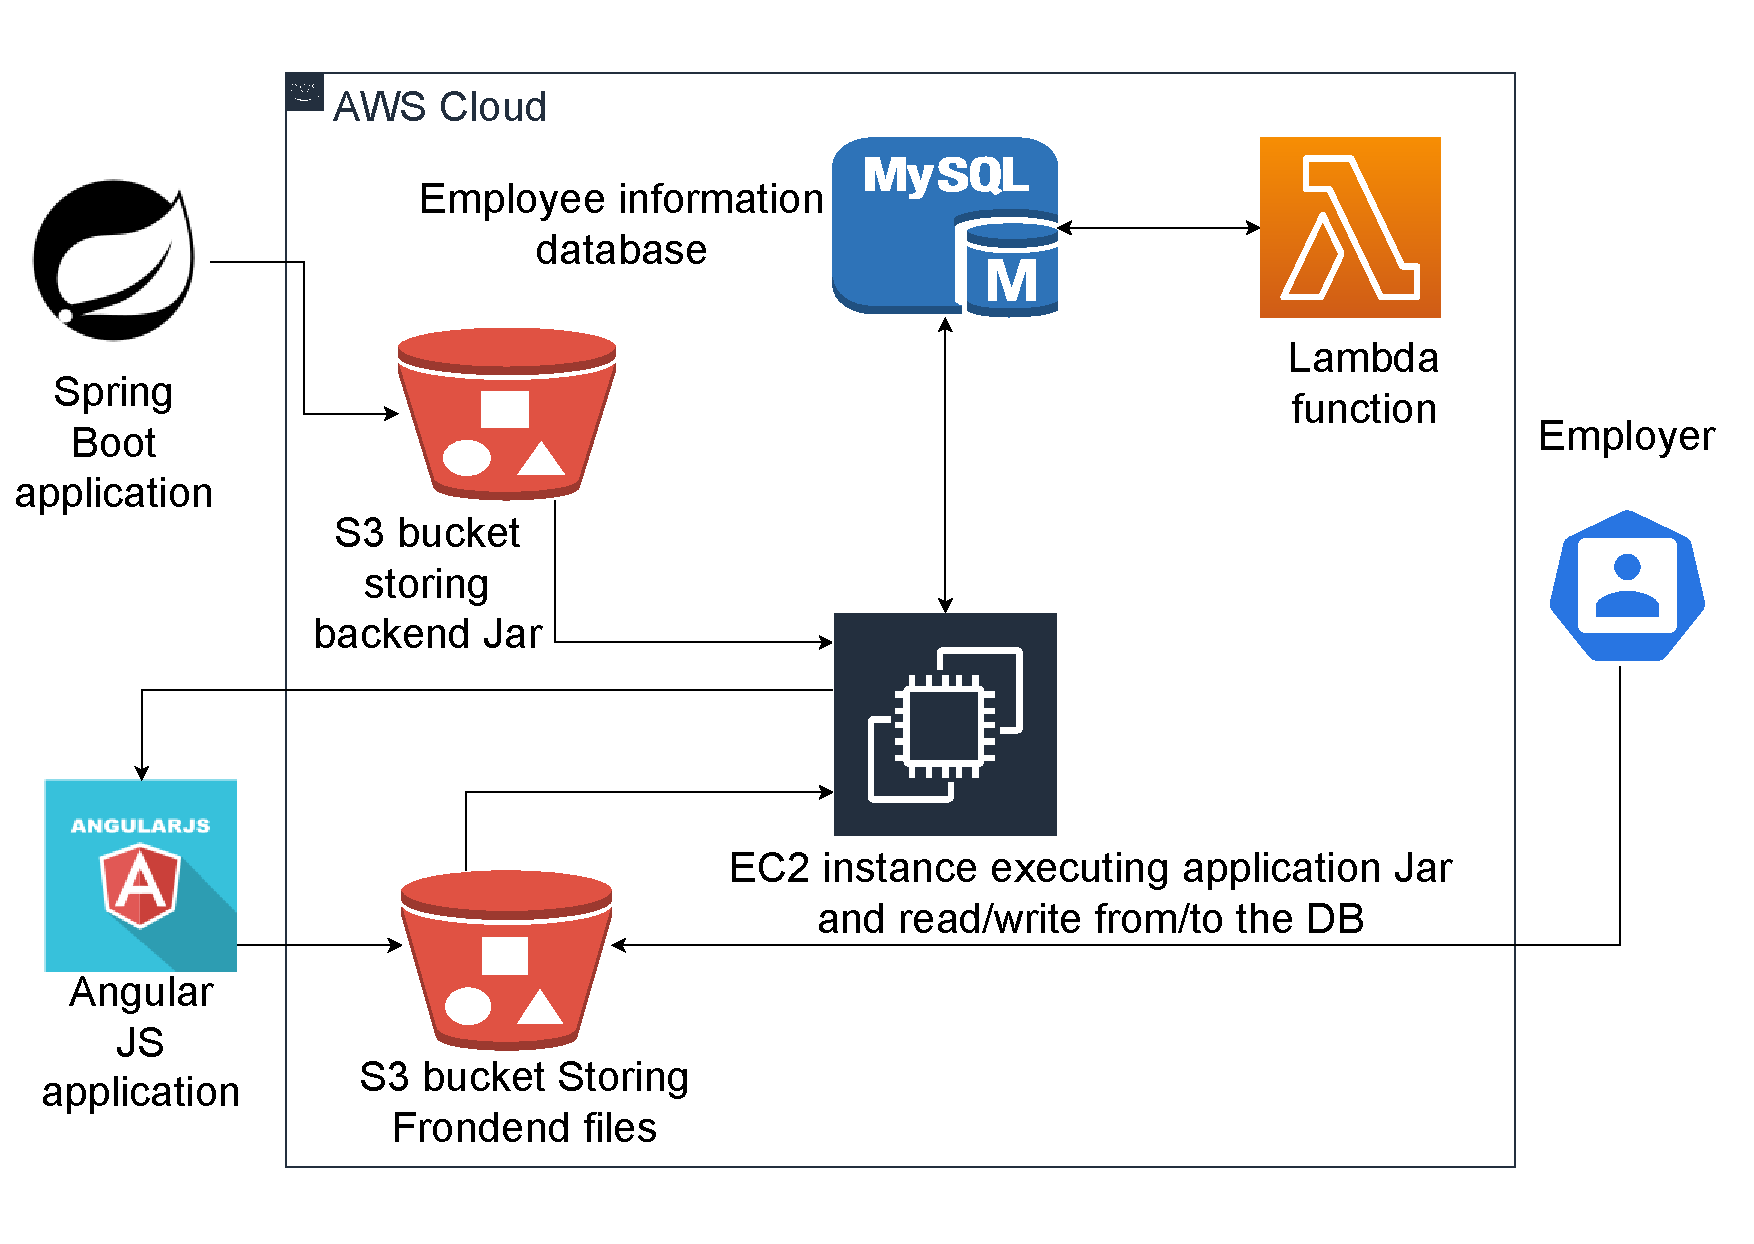
\includegraphics[width=\textwidth]{infrastructure_architecture.pdf}
    \caption{Infrastructure architecture}
    \label{fig:infrastructure_architecture}
\end{figure}

\par The architectural view of the open-source
application infrastructure is shown in the figure
\ref{fig:infrastructure_architecture}.
The application employs AWS services namely IAM, RDS, S3, EC2, and Lambda.
Below is a detailed explanation that helps to understand the role of each AWS service.

\par IAM

\par The application requires the creation of buckets, databases, ec2 instances, and lambda function and carries out the
execution of commands to perform security assessment
using Prowler and ScoutSuite \cite{79}.

\par To perform these operations, the user needs to be assigned the required permissions.
Based on the leave privilege principle the user should only be assigned the permission needed to perform the task.
If a user does not need an access right, then the user should not be assigned such access right \cite{80}.
AWS IAM service assigns the required permission to the user.
To create and write to the s3 bucket, the user is
assigned \textit{s3:CreateBucket} and \textit{s3:PutObject} permission \cite{81}.
To launch the ec2 instance, \textit{ec2:RunInstances}
permission is added to the user \cite{82}.
To create the database, \textit{rds:CreateDBCluster}
permission is assigned to the user \cite{83}.
To create and execute the lambda function,
\textit{lambda:CreateFunction} is added to the user \cite{84}.
\hfill \break
\par S3

\par The application backend of the employee management application as described above is developed in Spring boot and the frontend is developed in Angular.JS. The developed application is available in version control systems such as GitHub, Bitbucket, etc.
With the help of \gls{ci}/\gls{cd}, the application code is
deployed
in the AWS cloud.
CI/CD combines the practices of continuous integration and continuous delivery.
It helps the developers to make changes to code that are
then automatically tested and pushed out for delivery and
deployment \cite{85}.

\par The required application package, Jar in case of spring boot application, and modules in case of angular.js application are stored in S3 buckets.
For the application to be accessed by the HR or employer,
static web hosting is enabled for the bucket containing angular.js application files.


\hfill \break

\par RDS

\par Amazon RDS help to set up, run and scale database services in the cloud.
The employee management application enables adding, updating, and deleting the employee’s information.
This employee information is stored in the database.
The database details are added to the backend spring boot application which connects to the database to perform the required database operation in response to the request from the frontend angular application by making an API call.

\hfill \break
\par EC2

\par The S3 bucket stores the Java spring boot application jar.
The Jar contains the code implemented to perform different application operations.
For the web application to function, the backend application needs to be run.
To do so an EC2 instance is created.
The backend spring boot application jar is downloaded from the S3 bucket to the ec2 instance.
Once the Jar is downloaded, it is run on the EC2 instance
using the command \textit{java -jar applicationname.jar} 
\cite{78}.

\hfill \break
\par Lambda

\par Lambda services execute code without provisioning servers.
The application infrastructure contains a lambda function that makes an API call to the RDS database.
The function retrieves the information of employees within the organization.
The database details are hardcoded as a connection string within the lambda function.
Upon successful validation of the database details, the request is made to fetch the employee’s information.
\begin{figure}
    \centering
    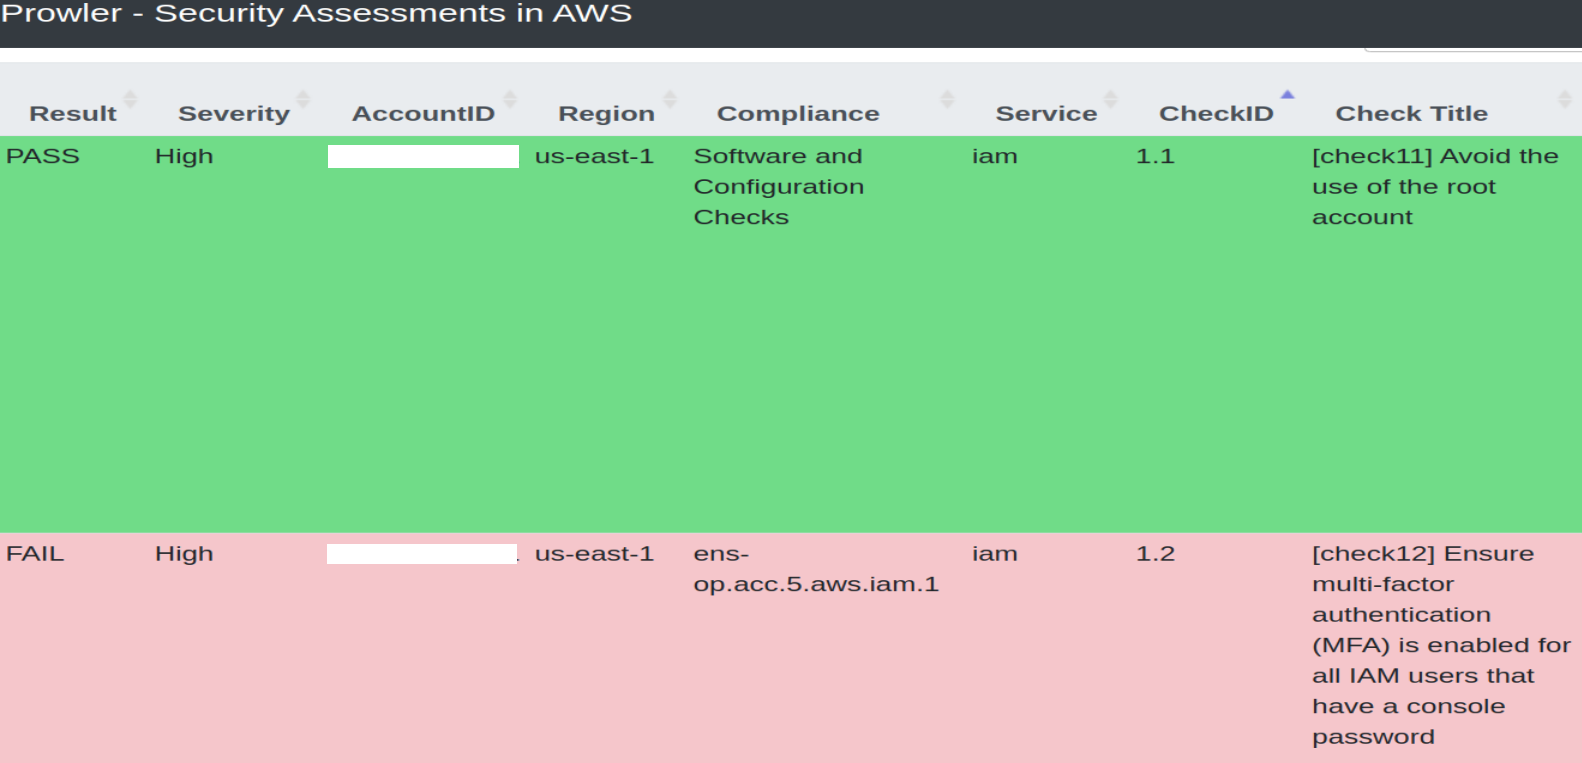
\includegraphics[width=175mm,height=12cm]{prowlerAssessment.PNG}
    \caption{Prowler security assessment}
    \label{fig:prowlerassessmentreport}
\end{figure}
\par To ensure the safety of the infrastructure, a security assessment needs to be performed to identify any security vulnerabilities that might have been introduced while setting up the infrastructure. This is performed by making use of security assessment tools such as Prowler. The assessment starts by executing the command \textit{./prowler}. Once the assessment completes, the assessment report is generated. This report provides details about the security vulnerabilities associated with different AWS services within the infrastructure.

Figure \ref{fig:prowlerassessmentreport} shows the snippet of the assessment report generated using Prowler.


\hfill \break
\section{ScoutSuite}

\par ScoutSuite is open-source tools used by external and
internal security analysts to perform the assessment of cloud environments.
It is used by external and internal security analysts to assess cloud environments.
To collect configuration data from high security risk areas for manual audit by researchers Scout Suite uses the API exposed by the cloud service provider.
Based on configuration gathered data, it shows security
risks and issues present in the infrastructure \cite{86}
\cite{87}.
\hfill \break
\par Features of ScoutSuite
\begin{itemize}
    \item Persistent monitoring: ScoutSuite is a user-friendly tool that provides the ability to constantly monitor
    the public cloud accounts.
    It helps to review computing resources in order to optimize the workflow by ensuring high performance and ceaseless service availability.
    It ensures tracking of the issues as they occur.
    Persistent monitoring also helps in the evaluation of
    program speed, resource availability, and resource
    levels, to help predict the security attack before it occurs \cite{88}.
\end{itemize}
\begin{itemize}
    \item Agnostic platform: Agnostic Platform refers to tools or applications that are compatible with any cloud
    infrastructure and can be moved without any operational issues to and from different cloud environments.
    An agnostic platform is similar to cloud-native tools which are platform specific and creates visibility issues businesses operating in a hybrid cloud or multi-cloud environment.
    Using cloud-agnostic tools such as ScoutSuite
    benefits from greater visibility across their cloud
    environment and gives them more clarity about how their ecosystem works, leading to better-informed decision making \cite{88}.
\end{itemize}


\hfill \break

\subsection{Deploying ScoutSuite}

\par Scout Suite is a multi-cloud tool namely \gls{gcp}
Google Cloud Platform, AWS, Microsoft Azure, etc.
In this research work, ScoutSuite is deployed on an AWS EC2 instance with an
IAM role configured \cite{87}.

\par Once the EC2 instance is running, the instance is connected.
Connection to the EC2 instance is established using EC2 Instance Connect, Session Manager, SSH client example Putty, and EC2 serial console.
After the EC2 instance is connected, it must be configured.
Configuring the environment can be done by running the
\textit{aws configure} command.
During configuration, it prompts for users access-key,
secret-key, output format and the region.
The user used to configure the environment must
be assigned the
ReadOnlyAccess and SecurityAudit AWS Managed Policies
\cite{87}.
Once configured, the virtual environment must be installed.
Installation of the virtual environment is done by using the command \textit{pip3 install virtualenv}.
After installing virtualenv, a virtual environment must be created, to do this the command \textit{virtualenv -p python3 venv} is executed.
The next step is to install ScoutSuite on the virtual environment.
Installing virtual environment requires running the commands \textit{source venv/bin/activate} and \textit{pip3 install scoutsuite}.
The final step is to test and run ScoutSuite.
Verification of the installation is done by running the command \textit{scout --help}.
The tool's usage syntax for different cloud environments is shown using the help command.
If the user wishes to use ScoutSuite against a specific
AWS IAM role, the command \textit{scout aws --profile my-aws-cli-profile} is executed.
The assessment of the AWS account against the security
vulnerabilities is started by executing the command\textit{scout aws}.
ScoutSuite gathers data from APIs, performs the authenticity of the configured environment variable, and pulls info on the cloud services and various resources.
Once Scout Suite finishes auditing the environment, an
HTML report will be generated \cite{87}.
Unlike checks in Prowler, ScoutSuite has rules.
To verify publicly accessible RDS instances, ScoutSuite uses the rule \textit{rds-instance-publicly-accessible}.
The result is demonstrated in table
\ref{tab:scoutsuiterule} \cite{88}.

\begin{table}[h!]
    \begin{center}
        \caption{ScoutSuite execution result}
        \label{tab:scoutsuiterule}
        \begin{tabular}{|p{1.4cm}|p{1.7cm}|p{5.0cm}|p{6.0cm}|}
            \hline
            \textbf{Result} & \textbf{Severity} & \textbf{Rule} & \textbf{Rule Title}\\
            \hline
            Good & Danger & rds-instance-publicly-accessible & RDS Instance publicly accessible \\
            \hline
        \end{tabular}
    \end{center}
\end{table}


Figure \ref{fig:deployscoutsuite} shows the snippet of
the report generated by using ScoutSuite.

\begin{figure}
    \centering
    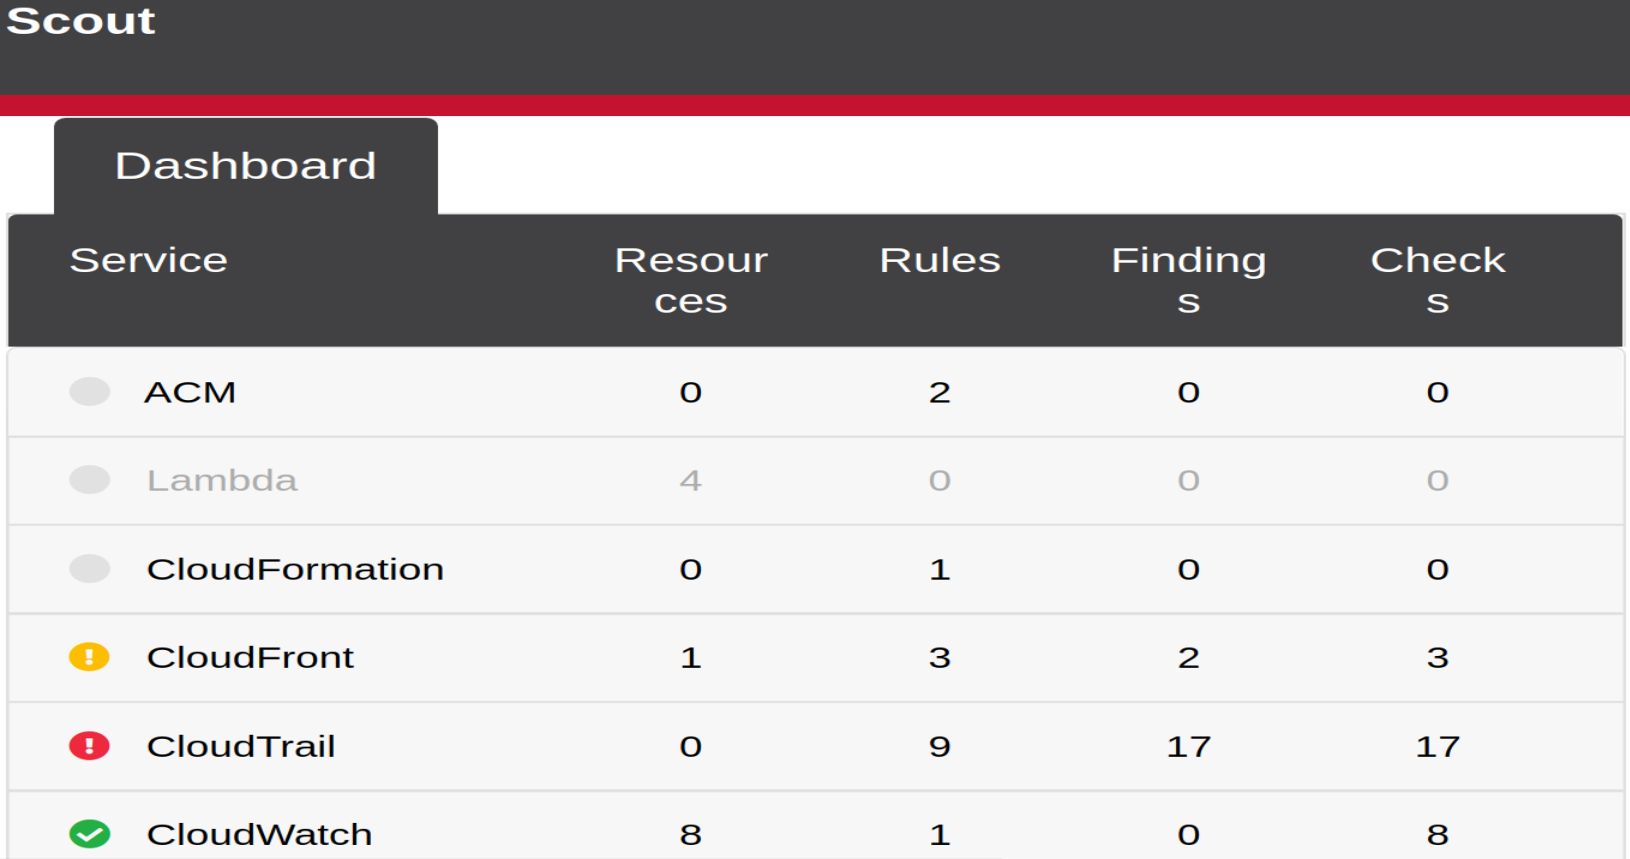
\includegraphics[width=\textwidth]{scoutAssessment.PNG}
    \caption{ScoutSuite Report}
    \label{fig:deployscoutsuite}
\end{figure}
%! Author = vsharma
%! Date = 25.09.2022
% !TeX spellcheck = en_EN

\chapter{Evaluation}

\par In this chapter, based on the approaches from the
previous chapter, the efficiency of
Prowler is evaluated against security vulnerabilities.
The result of the evaluation of each approach is discussed here.

\par In the end, a comparison between the assessment of security vulnerabilities performed using Prowler and
ScoutSuite is also highlighted which showcases the efficiency of each tool individually.

\section{Using Test Driven Approach}
\begin{figure}
    \centering
    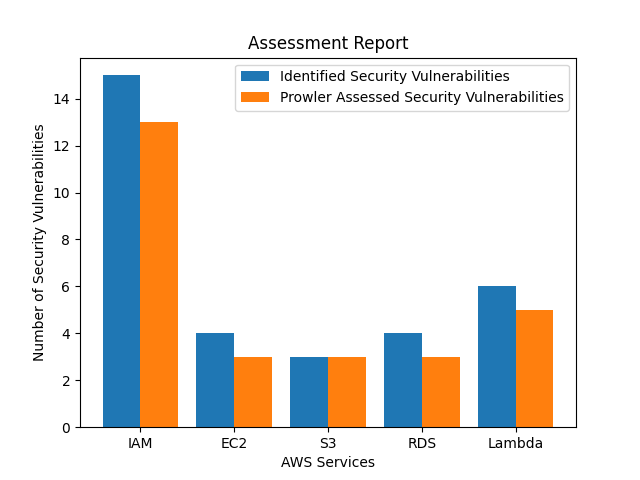
\includegraphics[width=\textwidth]{assessmentgraph.png}
    \caption{Prowler Assessment Graph}
    \label{fig:prowlerefficiency}
\end{figure}

\par The test-driven approach requires developing the test cases for the possible assessable scenario of a check in Prowler that performs the security assessment of an identified security vulnerability in the AWS service.
The individual test cases are developed, and their results are noted.

\par The checks in Prowler corresponding to the identified security vulnerabilities are identified manually.
The functionality of the check is understood and verified if the check can perform the assessment of the identified security vulnerability.
The verification process includes developing test cases for all assessable scenarios and evaluating the result of the assessment.
Only if all the scenarios are successfully verified the security vulnerability is marked to be assessed using Prowler.
Once all the test scenarios for the different checks in Prowler are developed and verified, the efficiency of Prowler is calculated against the identified security vulnerabilities for individual AWS services.
The efficiency calculation is done programmatically.

\begin{longtable}{|p{10cm}|p{2.4cm}|p{2cm}|}
    \hline
    \textbf{Security Vulnerabilities} & \textbf{Service} & \textbf{Prowler Check}\\
    \hline
    Avoid the use of the root account & IAM & Check11 \\
    \hline
    MFA is enabled for all IAM users & IAM & Check12 \\
    \hline
    Credentials unused for 90 days or greater are disabled & IAM & Check13 \\
    \hline
    Access keys are rotated every 90 days or less & IAM & Check14 \\
    \hline
    IAM password policy requires at least one uppercase letter & IAM & Check15 \\
    \hline
    IAM password policy requires at least one lowercase letter & IAM & Check16 \\
    \hline
    IAM password policy requires at least one symbol & IAM & Check17\\
    \hline
    IAM password policy requires at least one number & IAM & Check18\\
    \hline
    IAM password policy requires a minimum length of 14 or greater & IAM & Check19\\
    \hline
    IAM password policy prevents password reuse & IAM & Check110\\
    \hline
    IAM password policy expires passwords within 90 days or less & IAM & Check111\\
    \hline
    Password expiration requires an administrator reset & IAM & \\
    \hline
    Allow users to change their own password & IAM& \\
    \hline
    Insider Threat & IAM & Extra774\\
    \hline
    Access key for the root account & IAM & Check112 \\
    \hline
    Instances created from Malicious AMI & EC2 & Check76\\
    \hline
    User data public exposure & EC2 & Extra741\\
    \hline
    Server-Side Request Forgery & EC2 & Extra786\\
    \hline
    Denial of Wallet & EC2, Lambda &\\
    \hline
    Public exposure of S3 buckets & S3 & Check73\\
    \hline
    Unencrypted S3 buckets & S3 & Extra764\\
    \hline
    GhostWriter & S3 & Extra771 \\
    \hline
    Publicly accessible RDS instances & RDS & Check78\\
    \hline
    Unencrypted RDS Instance & RDS & Extra735\\
    \hline
    Resources running in an AWS classic resource & RDS & \\
    \hline
    Default data retention & RDS & Extra739\\
    \hline
    Lambda functions have a public resource-based policy & Lambda & Extra798 \\
    \hline
    Publicly accessible AWS account & Lambda & Extra7145 \\
    \hline
    Public lambda function URL & Lambda & Extra7179 \\
    \hline
    Public lambda function URL Cors & Lambda & Extra7180 \\
    \hline
    Insecure Management of Secrets & Lambda & Extra760\\
    \hline
    Poisoning the Well & Lambda & \\
    \hline
    \caption{Prowler Checks and mapped Security Vulnerabilities}
    \label{tab:securityvulnerabilitiescheckin prowler}
\end{longtable}

\par The process for calculating the efficiency of Prowler begins by determining the count of the security vulnerabilities that are identified for an AWS service.
The table \ref{tab:classificationofsecurityvulnerabilities} shows all the security vulnerabilities that are identified in the five AWS services.
Additionally, the table also highlights the different checks in Prowler that are identified and verified by developing the test cases that assess these identified security vulnerabilities.
The count of number of security vulnerabilities that are identified for the AWS service is determined.
Also, the number of security vulnerabilities that are assessed using Prowler for that AWS service is determined.
Based on these results the efficiency of Prowler is calculated in assessing an AWS service.
For example, looking at the table \ref{tab:classificationofsecurityvulnerabilities} and the graph \ref{fig:prowlerefficiency} considering AWS RDS, the number of identified security vulnerabilities is 4, and the number of security vulnerabilities that are assessed using Prowler is 3.
This process is performed for the 5 AWS services that are chosen for this research work.
In the end, it is possible to determine how efficient Prowler is in assessing the security vulnerabilities of each AWS service.


\par The graph \ref{fig:prowlerefficiency} is drawn between the AWS services considered for this thesis work and the number of security vulnerabilities.
It highlights the total number of security vulnerabilities identified for an AWS service and the number of security vulnerabilities that are assessed using Prowler for the AWS service.

\par Looking at the graph for IAM, it can be concluded that out of the 15 identified security vulnerabilities, Prowler performs the assessment of 13 security vulnerabilities.
The 2 security vulnerabilities that cannot be assessed by
Prowler are \textit{Password expiration requires
administrator reset} and \textit{Enabling account users
to set new password}.
These security vulnerabilities are caused due to excessive privilege.
The Password expiration requires an administrator reset feature prevents the user from updating their password after the account password has expired and thus requires administrative access.
This causes an issue on the user’s productivity and increases the workload on the administrator but ensures account safety.
If the account user is given administrative permission, this avoids the impact on the user’s productivity, but at the same time increases the risk that the user can cause.
This user can reset passwords for another user, revoke or grant unrestricted access to resources, files or directories and can even delete other user resources or accounts.
By enabling this features all the users to reset there
own account password.
If the user is granted an administrative role, the user would not just be able to change the password for his own account but would be able to manage other user accounts as well.
Assigning excessive privilege to a user can lead to 
deadly sin such as siphoning important information to the
competitors, data destruction, etc \cite{87}.

\par Like IAM, looking at the graph for EC2 it can be determined that out of the 4 identified security vulnerabilities, 3 of those security vulnerabilities are assessed using Prowler.
 The unassessed security vulnerability using Prowler is the Denial of wallet.
 Most of the time data loss incidents make the news, but the denial of wallet is one of the common ways that can be found out about a compromise through the AWS bill.
 The denial of wallet security vulnerability causes 
disruption of the target system or flooding the system 
with traffic as a form of threat, ransom, or revenge thus
depriving the system usage or leading to downtime 
resulting in loss of time and money, and reputation \cite{86}.

\par Prowler shows 100 \% efficiency in assessing the security vulnerabilities that are identified in S3 and thus Prowler is highly efficient in performing the security best practices assessments, audits, and incident response for S3.

\par Similar to IAM and EC2, out of 4 identified security
vulnerabilities prowler performs the assessment of 3 security vulnerabilities.
Prowler does not perform the assessment of security vulnerability that can occur due to RDS instances running on AWS classic resources.
The EC2-Classic platform is retired by Amazon and disabled on all accounts.
The EC2-Classic platform is replaced the EC2-VPC \cite{88}.

\par As seen from the graph \ref{fig:prowlerefficiency}, out of the 6 security vulnerabilities identified in AWS lambda, Prowler can perform the assessment of 5 security vulnerabilities.
The security vulnerability that is not assessed using Prowler is ‘Poisoning of well’.
Poisoning of well can be highly hazardous in numerous ways.
It can occur when the malicious users inject fake
training
data with the aim of corrupting the learned model and can
spread, affecting the products that draw from it or when
an Integrated Development Environment (IDE) plugin hosting the cloud server is controlled by an attacker.
A code backdoor is introduced as the security vulnerability by the attacker into the plugin \cite{89}.


\section{Using Open-Source Application}

\begin{figure}
    \centering
    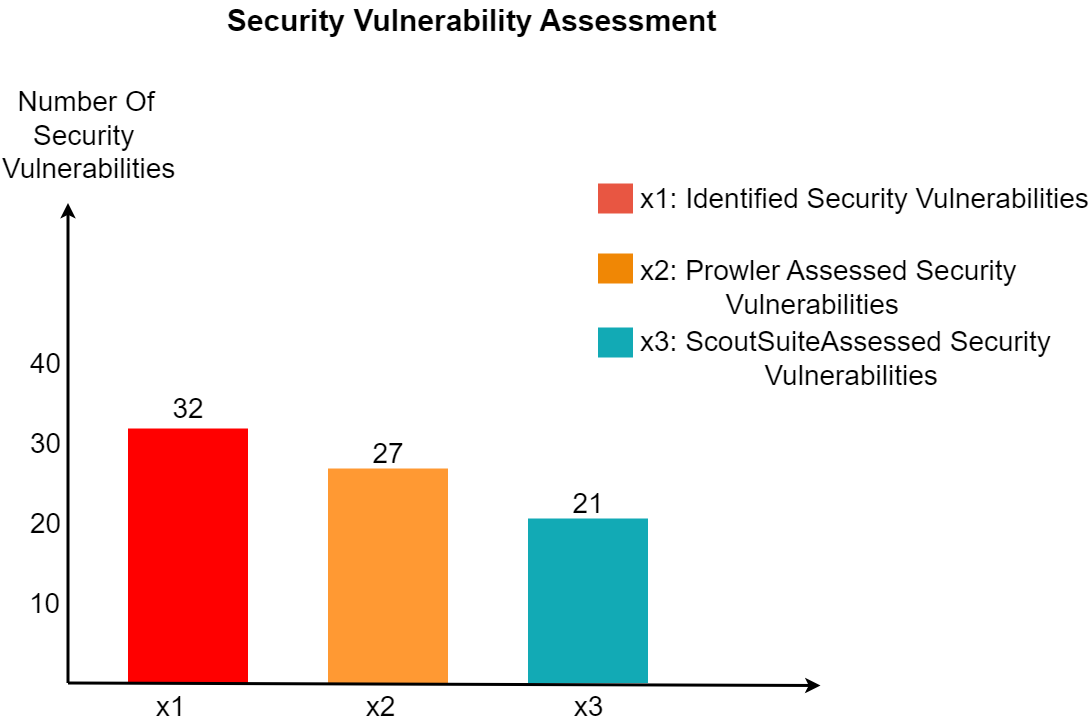
\includegraphics[width=\textwidth]{prowlervsscoutsuite.png}
    \caption{Security Vulnerabilities Assessment Graph}
    \label{fig:prowlervsscoutsuite}
\end{figure}

\par Cloud service providers make tools available to secure the cloud systems, but it is ultimately the user’s responsibility to use them.
The control needed to define and implement the cloud infrastructure differs greatly from the controls used in on-premises environments.
Simply transforming the hardware servers to AWS EC2 instances won't make the infrastructure secure by default.
This is because, while AWS is responsible for the
security of the cloud, it is the users responsibility
for the security in the cloud.
This resulted in organizations suffering from poorly architected and misconfigured cloud infrastructure leading to embarrassing data leaks \cite{74}.
This section shows the assessment of security vulnerability performed using two open-source cloud security assessment tools namely Prowler and ScoutSuite which can help strengthen the cloud security posture without breaking the bank.

\par The employee management web application \cite{69} leverages different AWS services namely IAM, EC2, S3, RDS, and Lambda for its deployment on AWS cloud infrastructure as shown in the figure \ref{fig:infrastructure_architecture}.
Once the application is deployed on the AWS cloud, the application functionality is verified.
The application provides different functions such as adding, updating and deleting the organization’s employee information.
As the application deployment takes place, there could be a chance of introduction of security vulnerability due to misconfiguration or security flaws within the application.
In order to deal with these issues, the AWS account must be assessed using the assessment tools against any security vulnerability that might have been introduced while deploying the application on the AWS infrastructure.

\par To assess the AWS account against any security vulnerabilities two security assessment tools namely Prowler and ScoutSuite were introduced in chapter 4.
To begin the assessment of the AWS account using Prowler the command \textit{./prowler} is executed, on the other hand, the assessment of security vulnerabilities using ScoutSuite is performed by executing the command \textit{scout aws}.

\par Once the assessment of the AWS account finishes, the assessment report is generated.
Prowler supports the generation of assessment reports in multiple formats such as text, CSV, JSON, JSON-ASFF, JUnit-XML, and HTML.
The generated assessment report provides a detailed 
description of the security vulnerability assessed, check
in Prowler that assesses the security vulnerability, the result of the assessment, region, associated AWS service, etc \cite{75}.
Similarly, when the assessment of the AWS account performed using ScoutSuite finishes, the assessment report is generated in PDF format.
The assessment report provides a descriptive view of the 
different AWS services, the resources leveraged by each 
service, the rules available for each service, etc \cite{76}.


\par \par Looking at the graph \ref{fig:prowlervsscoutsuite}, it can be inferred that a total of 32 security vulnerabilities are identified in five AWS services based on literatures, the Open Web Application Security Project (OWASP) vulnerability list \cite{43}, Cybersecurity \& Infrastructure Security Agency (CISA) \cite{42}, International Data Corporation (IDC) \cite{41} as shown in the table \ref{tab:securityvulnerabilitiesandresources}.
After the assessment of the AWS account finishes, a total of 27 of the identified security vulnerabilities are assessed using Prowler.
There are 5 security vulnerabilities that could not be assessed using Prowler as Prowler does not provide checks to assess those 5 security vulnerabilities.
Similarly, out of the 32 identified security vulnerabilities, ScoutSuite can perform the security assessment of 21 security vulnerabilities.
There are 11 security vulnerabilities that are not assessed using the rules provided by ScoutSuite.

\begin{longtable}{|p{9cm}|p{4.2cm}|}
    \hline
    \textbf{Security Vulnerabilities} & \textbf{Identification Resource}\\
    \hline
    Insider threat & Literature \cite{91} \\
    \hline
    Misconfiguration: & OWASP, CISA, IDC  \\
    \hline
    Instances created from Malicious AMI & Literature \cite{48} \\
    \hline
    User data public exposure & OWASP \\
    \hline
    Server-Side Request Forgery & OWASP \\
    \hline
    Denial of Wallet & CISA \\
    \hline
    Public exposure of S3 buckets & OWASP, Literature \cite{92}\\
    \hline
    Unencrypted S3 buckets & Literature \cite{93}\\
    \hline
    GhostWriter & CISA \\
    \hline
    Public RDS Database instance & OWASP\\
    \hline
    Resources running in AWS classic resources & Literature \cite{94}\\
    \hline
    Default data retention & Literature \cite{95} \\
    \hline
    Data Event Injection & OWASP \\
    \hline
    Insecure Management of Secrets & CISA\\
    \hline
    Poisoning the Well & CISA \\
    \hline
    \caption{Identified Security vulnerabilities}
    \label{tab:securityvulnerabilitiesandresources}
\end{longtable}

\par Based on the assessment of security vulnerabilities performed using the two security tools, it is possible to calculate the efficiency of the tools.
The formula to calculate efficiency of the two security assessment tools mathematically is the ratio of output to input expressed as a percentage \cite{88}.
\[ efficiency = (output/input) * 100 \]

Using this formula, the overall percentage efficiency of Prowler is calculated to be 84 \% and the overall efficiency of ScoutSuite is calculated to be 65 \%.

\par From the evaluated result for the two open-source security assessment tools can be inferred that Prowler possesses more checks than other tools miss.
It is a highly reliable and light piece of software with considerable documentation that helps developers and security auditors quickly set up and start security assessments.

\section{Comparision between Prowler and ScoutSuite}

\par In the previous sections of this chapter, the analysis was more manual-driven.
In the first approach, the test cases were developed for the different checks in Prowler and the efficiency was evaluated.
In the second approach, an open source was deployed on the infrastructure, and the infrastructure was assessed to perform the security assessment.
Based on the result of the assessment the efficiency was calculated.
\\
\par In this section, a real-world situation is considered.
An organization plans to migrate from its on-premises data center setup to the AWS cloud infrastructure.
Migration involves moving all the organization’s workload, data, and applications to the AWS cloud.
During the migration process, different AWS services are employed such as RDS, EC2, etc.
\\
\par After the migration of the organization's workload
to the cloud finishes, the organization plans to start using the cloud infrastructure in order to improve its customer experience.
Before starting to use the cloud infrastructure, a Security Engineer in the organization in a meeting advised performing a complete scan of the cloud infrastructure to avoid any security vulnerabilities that would have been introduced during the migration activity.
Considering the point made by the Security Engineer the company plans to perform a thorough scan of its cloud infrastructure.
\\
\par To begin this process, the cloud administrator creates a user account called \textit{audit-user}.
The audit-user is used to audit AWS cloud infrastructure.
During this process, the cloud infrastructure is assessed to identify any security vulnerability that would have been introduced while migrating the organization’s workloads to the cloud.
The cloud administrator plans to provide limited privileges to the audit-user to perform the assessment and verify different AWS services.
The table \ref{tab:accountconfiguration} shows the list
of policies assigned to the audit-user.
\\
\begin{longtable}{|p{6cm}|p{8cm}|}
    \hline
    \textbf{AWS Service} & \textbf{Managed Policy}\\
    \hline
    EC2 & AmazonEC2ReadOnlyAccess \\
    \hline
    S3 & AmazonS3FullAccess \\
    \hline
    Lambda & AWSLambdaBasicExecutionRole,
    AWSLambdaReadOnlyAccess \\
    \hline
    RDS & AmazonRDSReadOnlyAccess \\
    \hline
    \caption{AWS account configuration}
    \label{tab:accountconfiguration}
\end{longtable}



\par Once the audit-user account is provisioned with the required permission, the decision was made to use Prowler and ScoutSuite as the assessment tools to perform the assessment of the organization’s cloud infrastructure.
To perform the assessment using Prowler and ScoutSuite additional managed policies namely \textit{SecurityAudit} and \textit{ViewOnlyAccess} are assigned to the audit-user.

\par Before starting the assessment using the assessment tools, the audit-user plans to look at the different AWS services used for managing the organization’s workload.
During this process, the audit-user identifies a misconfiguration that was introduced while setting up the audit account.
The audit-user account was granted read-only permission
for EC2, Lambda, and RDS, but the audit-user was given \textit{AmazonS3FullAccess} to the S3 bucket.
Assigning full access to the S3 bucket for the audit-user account led to the deviation from the least privilege principle.
This permission grants the user full access to the S3 buckets.
The user can change the block public access setting, disable encryption of the bucket, and perform several other hazardous operations on the S3 buckets using this permission.

\par Once the audit-user finishes looking at the different AWS services, the audit-user plans to start the assessment of the cloud infrastructure using the two tools.
Before beginning the assessment, the audit-user configures the AWS cloud environment with the credentials.

\par Once the audit-user finishes looking at the different AWS services, the audit-user plans to start the assessment of the cloud infrastructure using the two tools.
Before beginning the assessment, the audit-user configures the AWS cloud environment with the credentials.
The audit-user starts the assessment by running the commands \textit{./prowler} and \textit{scout aws} to perform the assessment using Prowler and scout aws respectively.

\par After the assessment finishes, the assessment reports were generated.
The audit-user analyses the assessment report and identifies several security vulnerabilities in the cloud infrastructure.
There were EC2 Security groups that had ports exposed to all the sources addresses.
The ports should not be exposed publicly and if it is required to expose the port then a restriction on the source address must be made.
This would limit the surface of attacks on the cloud infrastructure.


\par On further analyses, it was found that the organization leverages two S3 buckets for storing files.
Based on the assessment report, it was found that for the S3 buckets logging was disabled.
Server logging should be enabled as it provides a detailed description of all the calls that were made to the bucket.
Also, it was found that multi-factor authentication (MFA) was not enabled for S3 bucket deletion.
Enabling MFA protects against unauthorized or accidental deletion of the S3 bucket.



\par In RDS, it was found that the RDS instance provisioned for storing the organization’s data had a single AZ configured.
Hence in case of loss of availability, the failover to
another instance would not possible.
Another security vulnerability related to AWS Lambda was identified.
A policy was attached to the Lambda function that allowed access to any AWS account.


\par Apart from the misconfiguration and security vulnerabilities highlighted above, the cloud infrastructure was assessed for the security vulnerability listed in chapter 4.
Based on the assessment performed using the two security
tools a table \ref{tab:comparisionresultprowlervsscoutsuite} comparing the assessment performed using the Prowler and ScoutSuite is created.

\begin{longtable}{|p{8cm}|p{2.4cm}|p{2cm}|p{2cm}|}
    \hline
    \textbf{Security Vulnerabilities} & \textbf{Service} & \textbf{Prowler} & \textbf{ScoutSuite}\\
    \hline
    Avoid the use of the root account & IAM & {{\color{green}\checkmark}} & {{\color{green}\checkmark}} \\
    \hline
    MFA is enabled for all IAM users & IAM & {{\color{green}\checkmark}} & {{\color{green}\checkmark}}\\
    \hline
    Credentials unused for 90 days or greater are disabled & IAM & {{\color{green}\checkmark}} & {{\color{green}\checkmark}}\\
    \hline
    Access keys are rotated every 90 days or less & IAM & {{\color{green}\checkmark}} & {{\color{green}\checkmark}}\\
    \hline
    IAM password policy requires at least one uppercase letter & IAM & {{\color{green}\checkmark}} & {{\color{green}\checkmark}}\\
    \hline
    IAM password policy requires at least one lowercase letter & IAM & {{\color{green}\checkmark}} & {{\color{green}\checkmark}}\\
    \hline
    IAM password policy requires at least one symbol & IAM & {{\color{green}\checkmark}} & {{\color{green}\checkmark}}\\
    \hline
    IAM password policy requires at least one number & IAM & {{\color{green}\checkmark}} & {{\color{green}\checkmark}}\\
    \hline
    IAM password policy requires a minimum length of 14 or greater & IAM & {{\color{green}\checkmark}} & {{\color{green}\checkmark}}\\
    \hline
    IAM password policy prevents password reuse & IAM & {{\color{green}\checkmark}} & {{\color{green}\checkmark}}\\
    \hline
    IAM password policy expires passwords within 90 days or less & IAM & {{\color{green}\checkmark}} & {{\color{green}\checkmark}}\\
    \hline
    Password expiration requires an administrator reset & IAM &  &\\
    \hline
    Allow users to change their own password & IAM & &\\
    \hline
    Insider Threat & IAM & {{\color{green}\checkmark}} & {{\color{green}\checkmark}}\\
    \hline
    Access key for the root account & IAM & {{\color{green}\checkmark}} & {{\color{green}\checkmark}}\\
    \hline
    Instances created from Malicious AMI & EC2 & {{\color{green}\checkmark}} & {{\color{green}\checkmark}}\\
    \hline
    User data public exposure & EC2 & {{\color{green}\checkmark}} & {{\color{green}\checkmark}}\\
    \hline
    Server-Side Request Forgery & EC2 & {{\color{green}\checkmark}} & \\
    \hline
    Denial of Wallet & EC2, Lambda & &\\
    \hline
    Public exposure of S3 buckets & S3 &  {{\color{green}\checkmark}} & {{\color{green}\checkmark}}\\
    \hline
    Unencrypted S3 buckets & S3 & {{\color{green}\checkmark}} & {{\color{green}\checkmark}}\\
    \hline
    Write access on S3 buckets (Ghostwriter) & S3 & {{\color{green}\checkmark}} & {{\color{green}\checkmark}}\\
    \hline
    Publicly accessible RDS instances & RDS & {{\color{green}\checkmark}} & {{\color{green}\checkmark}}\\
    \hline
    Unencrypted RDS Instance & RDS & {{\color{green}\checkmark}} & {{\color{green}\checkmark}}\\
    \hline
    Resources running in an AWS classic resource & RDS & &\\
    \hline
    Default data retention & RDS & {{\color{green}\checkmark}} & {{\color{green}\checkmark}}\\
    \hline
    Lambda functions have a public resource-based policy & Lambda & {{\color{green}\checkmark}} & \\
    \hline
    Publicly accessible AWS account & Lambda & {{\color{green}\checkmark}} & \\
    \hline
    Public lambda function URL & Lambda & {{\color{green}\checkmark}} &\\
    \hline
    Public lambda function URL Cors & Lambda & {{\color{green}\checkmark}} & \\
    \hline
    Insecure Management of Secrets & Lambda & {{\color{green}\checkmark}} &\\
    \hline
    Poisoning the Well & Lambda & & \\
    \hline
    \caption{Prowler vs ScoutSuite security vulnerability assessment}
    \label{tab:comparisionresultprowlervsscoutsuite}
\end{longtable}


\par Looking at the assessment results in the table \ref{tab:comparisionresultprowlervsscoutsuite}, it
is easy to determine how efficient individual security tools are in performing the security assessment of the security vulnerabilities associated with the different AWS services.

\par From the table, it is easy to understand the assessment performed for the different security vulnerabilities for each AWS service.
Starting with IAM, it can be inferred that both Prowler and ScoutSuite are equally efficient in performing the assessment of identified security vulnerabilities.
The two security vulnerabilities that were left unassessed by both tools occurs due to excessive privilege issue.
There is no check in Prowler, and there are rules in ScoutSuite to perform the security assessment of those security vulnerabilities.

\par For EC2, it can be seen that Prowler does not contain a check to assess Denial of Wallet security vulnerability, on the other hand, there are no rules in ScoutSuite to assess Server-Side Request Forgery and Denial of Wallet security vulnerabilities. SSRF attack can result in access to the configuration that includes files, metadata, etc. It scans the organization’s internal network, thus letting the malicious user exploit and identify unsecured services \cite{97}. The Denial of Wallet security vulnerability causes financial exhaustion to the organization \cite{86}.

\par It is seen that both tools were able to perform the assessment of all the identified security vulnerabilities in S3 and thus no security vulnerability is left unassessed.

\par Based on the assessment RDS, it is seen that the RDS instance running on AWS classic resource could not be assessed.
The AWS classic is retired by AWS and thus no checks or rules are available to perform the assessment \cite{88}.


\par ScoutSuite does not provide rules to access AWS Lambda \cite{72}, thus assessing the Lambda function is not possible using ScoutSuite.
Prowler performs the assessment of identified security vulnerabilities in AWS Lambda.
From the table \ref{tab:comparisionresultprowlervsscoutsuite}, it can be seen that Poisoning of Well is not assessed using Prowler as there are no checks available in Prowler to perform the assessment \cite{90}.
%! Author = vsharma
%! Date = 25.09.2022
% !TeX spellcheck = en_EN

\chapter{Conclusion and Future Work}

\par This chapter summarizes the thesis work and contribution, the overall evaluation results, and possible aspects of future work.

\section{Conclusion}

\par This research was aimed to identify and expose the security vulnerabilities of popular AWS Services.
It also aimed at investigating the efficiency of a security framework called Prowler in performing the assessment of security vulnerabilities.


\par Based on literatures, the \gls{owasp} vulnerability list \cite{51}, \gls{cisa} \cite{52}, \gls{idc} \cite{53} different security vulnerabilities in five AWS services were identified.
After identifying the different security vulnerabilities, the AWS cloud environment was assessed using Prowler to perform the assessment of these security vulnerabilities.


\par As part of this research work, the efficiency of Prowler was determined using two approaches.
The first approach was a test-driven manual approach, and the second approach used an open-source web application to determine the efficiency of Prowler.
Based on the number of security vulnerabilities assessed using Prowler, the efficiency of Prowler was calculated.
In both approaches, the efficiency of Prowler was
calculated to be greater than 80 \% with respect to the identified security vulnerabilities.


\par Apart from these two approaches, a use case of
an organization migrating its workload from an on-premises data center to an AWS cloud infrastructure was considered.
During the assessment of the newly set up cloud infrastructure using Prowler, several new security vulnerabilities and misconfigurations assessed using Prowler that were introduced during the migration to the AWS cloud were highlighted.

\par In addition to Prowler, another security assessment
tool called ScoutSuite was introduced.
The cloud infrastructure was accessed against the security vulnerabilities using ScoutSuite.
In the end, the assessment performed using Prowler and
ScoutSuite was compared.

\par Based on this research work, it can be concluded that Prowler is highly efficient in performing the security assessment of the identified security vulnerabilities.
It provides several checks for assessing different AWS services against security vulnerabilities.
Prowler generates the assessment result in multiple formats such as CSV, HTML, and JSON which enables integration with other tools, for example, Splunk.
It’s auditing, assessment, forensics readiness, and hardening capabilities make the AWS cloud infrastructure highly reliable and less vulnerable to incidents.


\section{Future Work}

\par Although this thesis work has explored the efficiency of Prowler in performing the assessment of security vulnerabilities, further studies are needed to confirm the obtained results.
More research should be done along with security experts from the industry in predicting the prominent security vulnerabilities and attacks in the referred five AWS services and other AWS services.


\par Another area for research could be to question companies using Prowler about their experience, determine
the pros and cons based on their experience, and identify
the limitations that the companies could face while using
Prowler.
\addcontentsline{toc}{chapter}{List of Figures}
\listoffigures
\addcontentsline{toc}{chapter}{List of Tables}
\listoftables
\addcontentsline{toc}{chapter}{List of Listings}
\lstlistoflistings

\addcontentsline{toc}{chapter}{List of Abbreviations}
\glsaddall

\printnoidxglossary[type=\acronymtype,style=long,
    title=List of Abbreviations,nonumberlist]

\addcontentsline{toc}{chapter}{References}
\bibliographystyle{ieeetr}
\bibliography{bibliography}

\end{document}
